\documentclass[letterpaper,12pt]{uoit_thesis}

\usepackage{amsmath,amssymb,amsthm,latexsym}
\usepackage{graphicx, subfigure}
\newtheorem{theorem}{Theorem}[section]
\usepackage{epstopdf}
\usepackage{url}
\usepackage[english]{babel}
\usepackage{hyperref}
%\usepackage{rotating}
%\usepackage{amsmath,epsf,psfig,epsfig}
%\usepackage{setspace}
%\usepackage[small,compact]{titlesec}
%\usepackage[mediumspace,mediumqspace,Grey,squaren]{SIunits}

%% Define a new 'leo' style for the package that will use a smaller font.
\makeatletter
\def\url@leostyle{%
  \@ifundefined{selectfont}{\def\UrlFont{\sf}}{\def\UrlFont{\small\ttfamily}}}
\makeatother
%% Now actually use the newly defined style.
\urlstyle{leo}

%\renewcommand{\label}{\textit{#1}}
%\usepackage[dvips]{graphicx}
%\usepackage{caption}
%\usepackage{subcaption}
%Comment these out when doing double-spaced submission version!
%\setlength{\parindent}{0pt}
%\setlength{\parskip}{1ex plus 0.5ex}

%\numberwithin{equation}{chapter}

\renewcommand{\baselinestretch}{1.5}
\newcommand{\ms}{\scriptscriptstyle\rm}

%\doublespace
\renewcommand{\baselinestretch}{1.5}


% Added by Jamil Jabbour
%differentiation
\makeatletter
\providecommand*{\diff}%
    {\@ifnextchar^{\DIfF}{\DIfF^{}}}
\def\DIfF^#1{%
    \mathop{\mathrm{\mathstrut d}}%
        \nolimits^{#1}\gobblespace}
\def\gobblespace{%
    \futurelet\diffarg\opspace}
\def\opspace{%
    \let\DiffSpace\!%
    \ifx\diffarg(%
        \let\DiffSpace\relax
    \else
        \ifx\diffarg[%
            \let\DiffSpace\relax
    \else
        \ifx\diffarg\{%
            \let\DiffSpace\relax
        \fi\fi\fi\DiffSpace}

%\providecommand*{\deriv}[3][]{%                   % \deriv[]{u}{x}
%   \frac{\diff^{#1}#2}{\diff #3^{#1}}}
\providecommand*{\deriv}[3][]{%                   % \deriv[]{u}{x}
    \frac{\diff^{#1}}{\diff #3^{#1}}#2}
\providecommand*{\pderiv}[3][]{%                  % \pderiv[2]{\psi}{x}
\frac{\partial^{#1}#2}%
{\partial #3^{#1}}}



% Added by Trevor
\renewcommand{\vec}[1]{\mathbf{#1}}
\newcommand{\pd}[2]{\frac{\partial #1}{\partial #2}}
\newcommand{\tx}[1]{\mathrm{#1}}
\newcommand{\rcite}[1]{\textcolor{red}\cite{#1}}
\newcommand{\axr}[1]{*** \textcolor{red} {#1} *** }
\newcommand{\axb}[1]{*** \textcolor{blue} {#1} *** }

\newcommand{\refb}[1]{(\ref{#1})}
\newcommand{\ds}{\displaystyle}
\newcommand{\beq}{\begin{equation}}
\newcommand{\eeq}{\end{equation}}
\newcommand{\beqa}{\begin{eqnarray}}
\newcommand{\eeqa}{\end{eqnarray}}
\newcommand{\bea}{\begin{array}}
\newcommand{\eea}{\end{array}}

\newcommand{\been}{\begin{enumerate}}
\newcommand{\een}{\end{enumerate}}
\newcommand{\beit}{\begin{itemize}}
\newcommand{\eeit}{\end{itemize}}

\renewcommand{\O}{\mbox{$\mathbf{O}$}}
\def\lb{\left(}
\def\rb{\right)}
\def\LB{\left[}
\def\RB{\right]}
\def\Lb{\left\{}
\def\Rb{\right\}}
\def\la{\langle}
\def\ra{\rangle}
\def\dl{\partial}
\def\nb{\nabla}
\def\vp{\varphi}


\begin{document}

% Preliminary pages
\makepreliminaries

\figurespagetrue
\tablespagetrue

\title{A Matrix-free numerical bifurcation method applied to sheared annular electroconvection}
\author{Jamil Antoine Jabbour}
\submitiondate{August 14, 2015}
\date{\today}
%\wordcount{58764 words}
\titlepage
%\cleardoublepage

\prefacesection{Abstract}
%\vspace{-1.5cm}
We investigate the flow transitions in sheared annular electroconvection using {matrix-free} numerical bifurcation methods. In particular, we study a model that simulates a liquid crystal film in the Smectic~A phase suspended between two annular electrodes, and subjected to an electric potential difference and a shear applied by rotating the inner anode at a constant rate.
Due to the Smectic A nature of the liquid crystal, the fluid can be considered two-dimensional and is modelled using the 2-D incompressible {Navier-Stokes} equations coupled with an equation for charge continuity. The charge density and the electric potential are coupled using a nonlocal relation given by Maxwell's equations.

%In this thesis, dynamical system approach is used to identify the transition of the flow, by implementing numerical bifurcation methods.
In this thesis, a {matrix-free} numerical bifurcation method is implemented to identify the transitions of the flow that result due to changes in the main nondimensional control parameter, the Rayleigh number $\mathcal{R}$, which is proportional to the square of the applied voltage. %Upon increasing $\mathcal{R}$, the flow undergoes successive transitions from the axisymmetric base state, to rotating waves, to amplitude vacillating waves. %A pseudo-spectral method has been implemented in MATLAB that numerically integrates perturbations from the base state.Rayleigh number $\mathcal{R}$.
This method consists of a natural continuation method that computes the axisymmetric and rotating waves state by detecting fixed points of two different discrete-time dynamical systems based on numerical integration, and a linear stability analysis that identifies the local behaviour of the flow.
%In the numerical bifurcation method, the Jacobian of the nonlinear system is approximated using finite differences. This leads to the use of matrix-free methods to solve the linear system obtained at every Newton iteration as well as the eigenvalue problem.Due to the $SO(2)$ symmetry of the system, a different approach is implemented to compute the rotating wave state. The techniques of implementation are presented and the results are summarized in a bifurcation diagram where the primary and secondary transitions are captured.
The nature of the rotating waves is used to simplify the computation of their corresponding solutions.
The primary transition from axisymmetric flow to rotating waves, and the secondary transition from rotating waves to amplitude vacillation are isolated. The results are consistent with previous experimental results and numerical simulations, and are summarized in a numerically computed bifurcation diagram.

\cleardoublepage

\prefacesection{Acknowledgements}

To start with, I would like to express my special thanks of gratitude to my Supervisor Dr.\ Greg Lewis for his time, tremendous support, and guidance. You have been a wonderful supervisor for me. I would like to thank you for encouraging my research and allowing me to be acquainted with so many new and innovative things.
I would like to express my gratitude to Dr.\ Sean Bohun, Dr. Lennaert van Veen, Dr.\ Pietro-Luciano Buono and Dr.\ Dhavide Aruliah for their useful comments, remarks and engagement through the learning process of this MSC. thesis. I would like to thank Dr.\ Stephen Morris for introducing the electroconvection model, Dr.\ Mary Pugh and Dr.\ Peichun  Tsai for sharing the numerical time solver codes.
Secondly, I would like to thank my parents and fianc\'ee for their support throughout the entire process, both by keeping me harmonious and encouraging me to focus on my research in any way possible.
Furthermore, I would like to acknowledge my colleagues and friends for their supportive attitude, encouragement and valuable commentaries and suggestions which provided me the incentive to strive towards my goal. I also thank the Ontario Ministry of Training, Colleges, and Universities for the Ontario Graduate Scholarship which funded me during the first year of my MSC. program.
Lastly, I would like to be grateful of University of Ontario Institute of Technology for accepting me into their Master’s program, providing me with a place to work in comfort, and for offering me opportunities such as teaching assistantships to support me financially.


%\cleardoublepage

\declarationpage

%\cleardoublepage

\contents

\afterpreliminaries


\pagenumbering{arabic}

\chapter{Introduction}
\thispagestyle{empty}
In many fluid systems, flow transition phenomena occur due to a change in a \emph{control} parameter, where the fluid motion is self-organized in patterns which depend on the symmetry in the system. The changes in the control parameter can lead to instability which can drive the system out of one equilibrium state and into another, eventually leading to chaos. It is of interest to understand these critical conditions under which transitions occur, and many classical examples which exhibit such transitions, have been studied extensively.
%In \emph{Poiseuille flow}, transition  from laminar to turbulent flow in a circular pipe arises due to a critical speed in the center of the pipe \cite{Pois_tran,Poi_sub_tran}.
With infinite parallel plates heated from below, the transition from pure conduction to  \emph{Rayleigh-B\'enard} convection occurs at a critical temperature difference between the plates.
Another classical example is the differentially heated co-rotating cylinders, which has been employed to model {large-scale} geophysical fluids ~\cite{Lew_Henn,Lew_DoubleHopf}. The fluid flow between the cylinders undergoes successive transitions from axisysmmetric flow to steady waves, to amplitude vacillating waves, to more irregular flows  upon increasing the temperature difference between the rotating boundaries and/or the rotation rate of the cylinders.

In this thesis, the fluid system of interest is sheared annular electroconvection. This situation is analogous to a {two-dimensional} version of the  differentially heated co-rotating cylinder system, where the transport of charge and the electric body force resulting from an applied electric potential are analogous to the transport of heat and the buoyancy force due to the temperature differences, respectively. The crucial difference is in the choice of fluid, i.e. a liquid crystal in {Smectic A} phase, which essentially can be considered a {2-D} fluid. It is of intrinsic interest to study this system which is capable of providing insight into transition phenomena in buoyancy driven rotating flows.

To obtain a better understanding of the transitions of the flow in sheared annular electroconvection, experimental and numerical methods have previously been undertaken.
Experimental results have been reported by Morris \& de Bruyn~\cite{mao1995,morris1992,experi_elec} beginning with the visualization of \emph{Rayleigh-B\'enard} convective cells in rectangular geometry. In the case of annular flow, results have been generated with a laboratory setup consisting of a thin liquid crystal film suspended between two annular electrodes with the inner anode rotating at a constant rate. In this experiment, control parameters such as the potential difference, the distance between the two electrodes, and the angular rate of the inner electrode can be varied. Under small electric potential difference, the system exhibits axisymmetric flow, in which the velocity of the fluid is in the azimuthal direction and the charge diffuses between the boundaries. At a critical potential difference, a primary transition occurs to rotating waves in which the charge is convected by the flow. Beyond this potential difference, it is observed that the system  undergoes successive transitions from the rotating wave state, to amplitude vacillating waves, to irregular flow.

%Smectic electroconvection begins with the experimental work of Morris \cite{mao1995,morris1992,experi_elec} and the visualization of \emph{Rayleigh-B\'enard} convective cells in rectangular geometry.

Using the experimental results as a backdrop, the sheared annular electroconvection system was modelled with a system of partial differential equations (PDEs) and algebraic equations (AEs) which were subsequently analyzed~\cite{EDCTAFUCF,BAEWIS,AEWSDaDe,linearstability,WNAEISFF,Annular}.
%developed the analytical base solution and performed an analysis of the resulting partial differential equations (PDEs) and algebraic equations (AEs) that model the annular electroconvection.
Up to this point in the literature, the focus has been on the primary flow transition from the axisymmetric base state to the rotating waves.
Subsequently Tsai and coworkers~\cite{PeiChunTsain,DNSSAE,tsai2004aspect,LSSE-PeDa} developed a numerical solver for the full model. In that work, the model equations are  integrated forward in time and the evolution of the physical quantities is observed for a small set of initial conditions varying values of the control parameters. We refer to such methods collectively as numerical experimentation.  Using this method, Tsai~et~al.~\cite{PeiChunTsain,DNSSAE} observed that the axisymmetric flow undergoes a sequence of transitions as the Rayleigh number is increased, eventually resulting in a chaotic regime. Tsai's observations were consistent with earlier analysis that predicted that the primary transition is a supercritical Hopf bifurcation~\cite{linearstability}. However, numerical experimentation is not able to compute unstable flows, nor is it able to accurately determine transition points, or determine the type of bifurcation associated with the transition. Therefore, due to the limitations of the method, the nature of the transitions could not be verified.

Alternative methods can be used to compute the asymptotic behaviour of solutions as parameters of the model are changed.    Possible asymptotic states of the flow may include steady states, periodic orbits, {quasi-periodic}, invariant tori or other more complex invariant limit sets. Finding the transition due to critical conditions can be rephrased in the language of dynamical systems theory as finding the critical parameter values at which bifurcations in the flow state occur. Practical methods for computing the transitions are known collectively as numerical bifurcation methods (NBMs) which consist of continuation methods that identify certain asymptotic sates and a linear stability analysis that investigates their local behaviour. The NBMs have advantages over the numerical experimentation method due to the systematic and unambiguous computation of the equilibria and bifurcations. They are able to compute unstable solutions as well as solutions exhibiting {bi-stability} without knowledge of the initial conditions that lead to these solutions, and thus are able to provide a clearer picture of the dynamics of the system. Moreover, they provide insight into the underlying physics that governs transition in the flow. However, the advantages of this approach is balanced by the sophisticated linear algebra required in its implementation.

In this thesis, we present a numerical bifurcation analysis of the sheared annular electroconvection problem. In particular, a matrix-free method based on numerical integration of the model equations is implemented to compute steady states and limit cycles, which correspond to the axisymmetric flow and rotating waves, respectively. In the matrix-free approach, these solutions can be computed as fixed points of two different discrete dynamical systems. This is possible in the case of rotating waves because we take into account that they are a special type of limit cycle. In particular, they are waves of constant amplitude that rotate at a constant phase speed.  The development and implementation of the matrix-free method for the computation of rotating waves represents the main original contribution of this thesis. With this method, we resolve the secondary transition in the sheared annular electroconvection problem, complimenting the work of Tsai~et~al.~\cite{EDCTAFUCF,BAEWIS,AEWSDaDe,linearstability,WNAEISFF,Annular}.

In Chapter 2, we provide details of the electroconvection experiment and of the mathematical and numerical models used to study it. We also discuss previous numerical and experimental results. In Chapter 3, we introduce the matrix-free methods used in the thesis, and discuss some details of the implementation. These methods provide an advantage over the more common methods used in various software packages such as MATCONT and AUTO~\cite{MATCONT}, in particular, by framing the computation in a way that does not require the storage of large matrices. We also expand upon these advantages in Chapter 3. The results and a comparison to previous work are presented in Chapter 4. Finally, the thesis closes with some reflections on the progress that has been made with an eye towards future work utilizing numerical bifurcation methods for computing more complex flows.

%The aim of this thesis is to give an overview of the implemented matrix-free numerical bifurcation methods; in particular a different approach is carried out to compute limit cycles using integration-time map, where the rotating waves are computed directly for general periodic orbit discussed in Chapter 3. The advantages of this approach over the standard approach that is used in different packages such as MATCONT and AUTO ~\cite{MATCONT} arise in solving a much more reduced system as well as the use of matrix-free algorithms. The implemented methods are tested on the sheared annular electroconvection and this is developed in Chapter 2. Finally, Chapter 4 presents the results achieved through-out the research with a comparison to previous results. The main contribution is a new approach developed to compute the flow of rotating waves. In the case of the electroconvection flow, this techniques was able to resolve the secondary transition extending the work of Tsai.
%The thesis closes with some reflections on the progress that have been made with an eye towards future work utilizing numerical bifurcation methods with more complex flow.

%\section{Contributions}
%In this thesis, the initial value solver of the perturbation equations from the base state of the sheared annular electroconvection implemented by (Tsai \cite{PeiChunTsain}) is modified and tailored to the computation needed and is used as a black box in our matrix-free numerical bifurcation method. This method is implemented in MATLAB to trace two type of invariant limit sets (steady states and limit cycles) of a dynamical system. The results of our computation of steady states and the primary bifurcation is compared and validated with the previous experimental \cite{experi_elec}, analytical \cite{linearstability} and numerical results \cite{EDCTAFUCF,SBSAE,DNSSAE} performed.
%A different approach is implemented to compute limit cycles corresponding to the flow of rotating waves \cite{rel_equ}, that is, the phase speed of the rotating wave is computed instead of the period. Using this technique, the degree of freedom are reduced extensively from the approach that requires to compute the period. The solution curve corresponding to the flow of rotating waves is traced and the secondary bifurcation point is determined for the first time using linear stability analysis.



%
%This thesis develops a matrix-free bifurcation method which is able to classify two types of invariant limit sets, (steady states and limit cycles). Using the newly developed method, we can compute the asymptotic behaviours of the equilibrium solution as parameters of the model are changed.

\chapter{Electroconvection}\label{ch_ele}
The term ``Electroconvection'' refers to the phenomena that occurs when a moving electrically susceptible fluid
is subjected to an applied electric field. Various geometries have been considered in the literature including, rectangular~\cite{linearstability,WNAEISFF,pattern}, annular~\cite{Annular}, and sheared annular~\cite{EDCTAFUCF,BAEWIS,SBSAE,AEWSDaDe}.
In this thesis, we consider this last case. In particular, we consider an experiment that involves a thin conductive crystal fluid in the Smectic~A phase suspended between two concentric annular electrodes. The inner electrode is rotated at a constant speed $\omega_{i}$, imposing a radial shear, and a DC voltage $V$ is applied between the two electrodes. This chapter presents an overview of the experiment of sheared annular electroconvection  and the governing equations that model it. In Section~\ref{sec_num_sol}, we present a brief overview of the simulation code that will be used in the numerical bifurcation method; for more details about the code and its implementation, we refer the reader elsewhere~\cite{PeiChunTsain}.

\section{The Physical Experiment}\label{sec_phy_exp}
We begin by introducing the experiment of Morris~et~al.~\cite{AEWSDaDe}; we include a brief description of its procedure and apparatus which has been designed to perform current-voltage measurements of electroconvection in annular liquid crystal films.
The experiment consists of observing a weakly conducting, sub-micron thick, liquid crystal film freely suspended between two concentric electrodes as the control parameters are varied. The entire set up is enclosed in an aluminum box which serves as a Faraday cage to reduce external electric interference. In the experiment setup, a razor blade controlled by a motor draws the film across the annular gap, and the electrodes are made concentric and levelled by a translation of the stage on which the fluid is suspended, by tilting adjustment rods, respectively.
Using a high precision electrometer controlled by a computer, a DC voltage $V$ is imposed across the electrodes and the resulting current $I$ is measured.
The main interest of the experiment is to study the charge transport by measuring the current $I$  as the fluid undergoes transitions as the voltage $V$ is varied.

\subsection{The fluid material}
The fluid used in the experiment is 8CB (4-cyano-4'octylbiphenyl)~\cite{AEWSDaDe}. Below $21.5^{\circ}$C, 8CB exhibits the spatial structure of a solid crystal with long-range positional and rotational order, while at temperatures higher than $40.5^{\circ}$C, the compound becomes spatially randomized and behaves as a liquid. Between these temperatures, 8CB exhibits a liquid crystal state. A schematic of the chemical formula of the fluid and the phases that it exhibits at different temperature is illustrated in Figure~\ref{8CB}, and the molecular arrangements are shown in Figure~\ref{smectic}.
Liquid crystal matter can be classified depending on the amount of order in the material~\cite{book2012liquid}. Between the temperatures $33.5^\circ$C and $40.5^{\circ}$C, 8CB exhibits a nematic phase characterized by molecules with no positional order but that point in the same direction. At lower temperatures, between $21.5^{\circ}$C and $33.5^{\circ}$C, the material enters a Smectic~A phase, where a degree of translational order is present.  In this phase, the molecules are maintained in a general orientation normal to the plane of the film and align themselves in an integer number of layers. Between the layers, motion is restricted. However, within each layer, the oriented molecules are free to move with no long-range order. Thus, each layer acts as a two-dimensional fluid.

\begin{figure}[tbh]
\centerline{\includegraphics[width =0.9\textwidth]{./figures/Pictures/8CB.png}}
\caption{Chemical formula and phase sequence of 8CB as its temperature changes.}
\label{8CB}
%[Chemical formula of 4-cyano-4'octylbiphenyl (8CB)]
\end{figure}

\begin{figure}[tbh]
%\centerline{\includegraphics[width =0.25\textwidth, keepaspectratio]{./figures/smecticphase.png}}
\centerline{\includegraphics[width =0.9\textwidth]{./figures/Pictures/liquid_crystal.png}}
\caption{Illustration of the liquid crystal that form the nematic (b) and smectic (c) phases upon cooling from the isotropic liquid (a) and above the crystal structure (d), adapted from~\cite{book2012liquid}.}
\label{smectic}
%[Changes of liquid crystal phase as temperature varies]
%\caption{shows the liquid crystal molecules in smectic-A phase. The molecules on an average are aligned in an integer number of layers with a particular normal direction. }
\end{figure}

The experiments which we will study  were conducted at room temperature $24\pm 2^{\circ}$C and atmospheric pressure. Thus the compound 8CB is in the Smectic~A phase.

\subsection{Experimental results}
A standard experiment consists of incrementing the applied voltage from $0$ volts to $1000$ volts and then decrementing it back to $0$ volts in small steps, with the inner anode rotating at a prescribed constant angular speed $\omega_i$ and the outer cathode stationary and grounded. For the range of rotation rate used in the experiments, the fluid is axisymmetric for relatively low voltage. In this state, the velocity is in the azimuthal direction where the flow lines are concentric circles and the charge diffuses between the electrodes by conduction. However, when the applied voltage $V$ exceeds a critical voltage $V_c$, the fluid becomes arranged into convective pairs of symmetric vortices, and the flow of electric charge between the electrodes constitutes a convective electric current. A snapshot of the fluid in these two states is illustrated in Figure~\ref{fig_exp_snap}.
At higher voltages $V > V_c$, a more complicated flow is provoked which retains large-scale structure of the convecting vortices. Thus, quantitative data are obtained, analysed and subsequently interpreted from raw experimental current-voltage measurements.
\begin{figure}[th]
\begin{center}
\subfigure{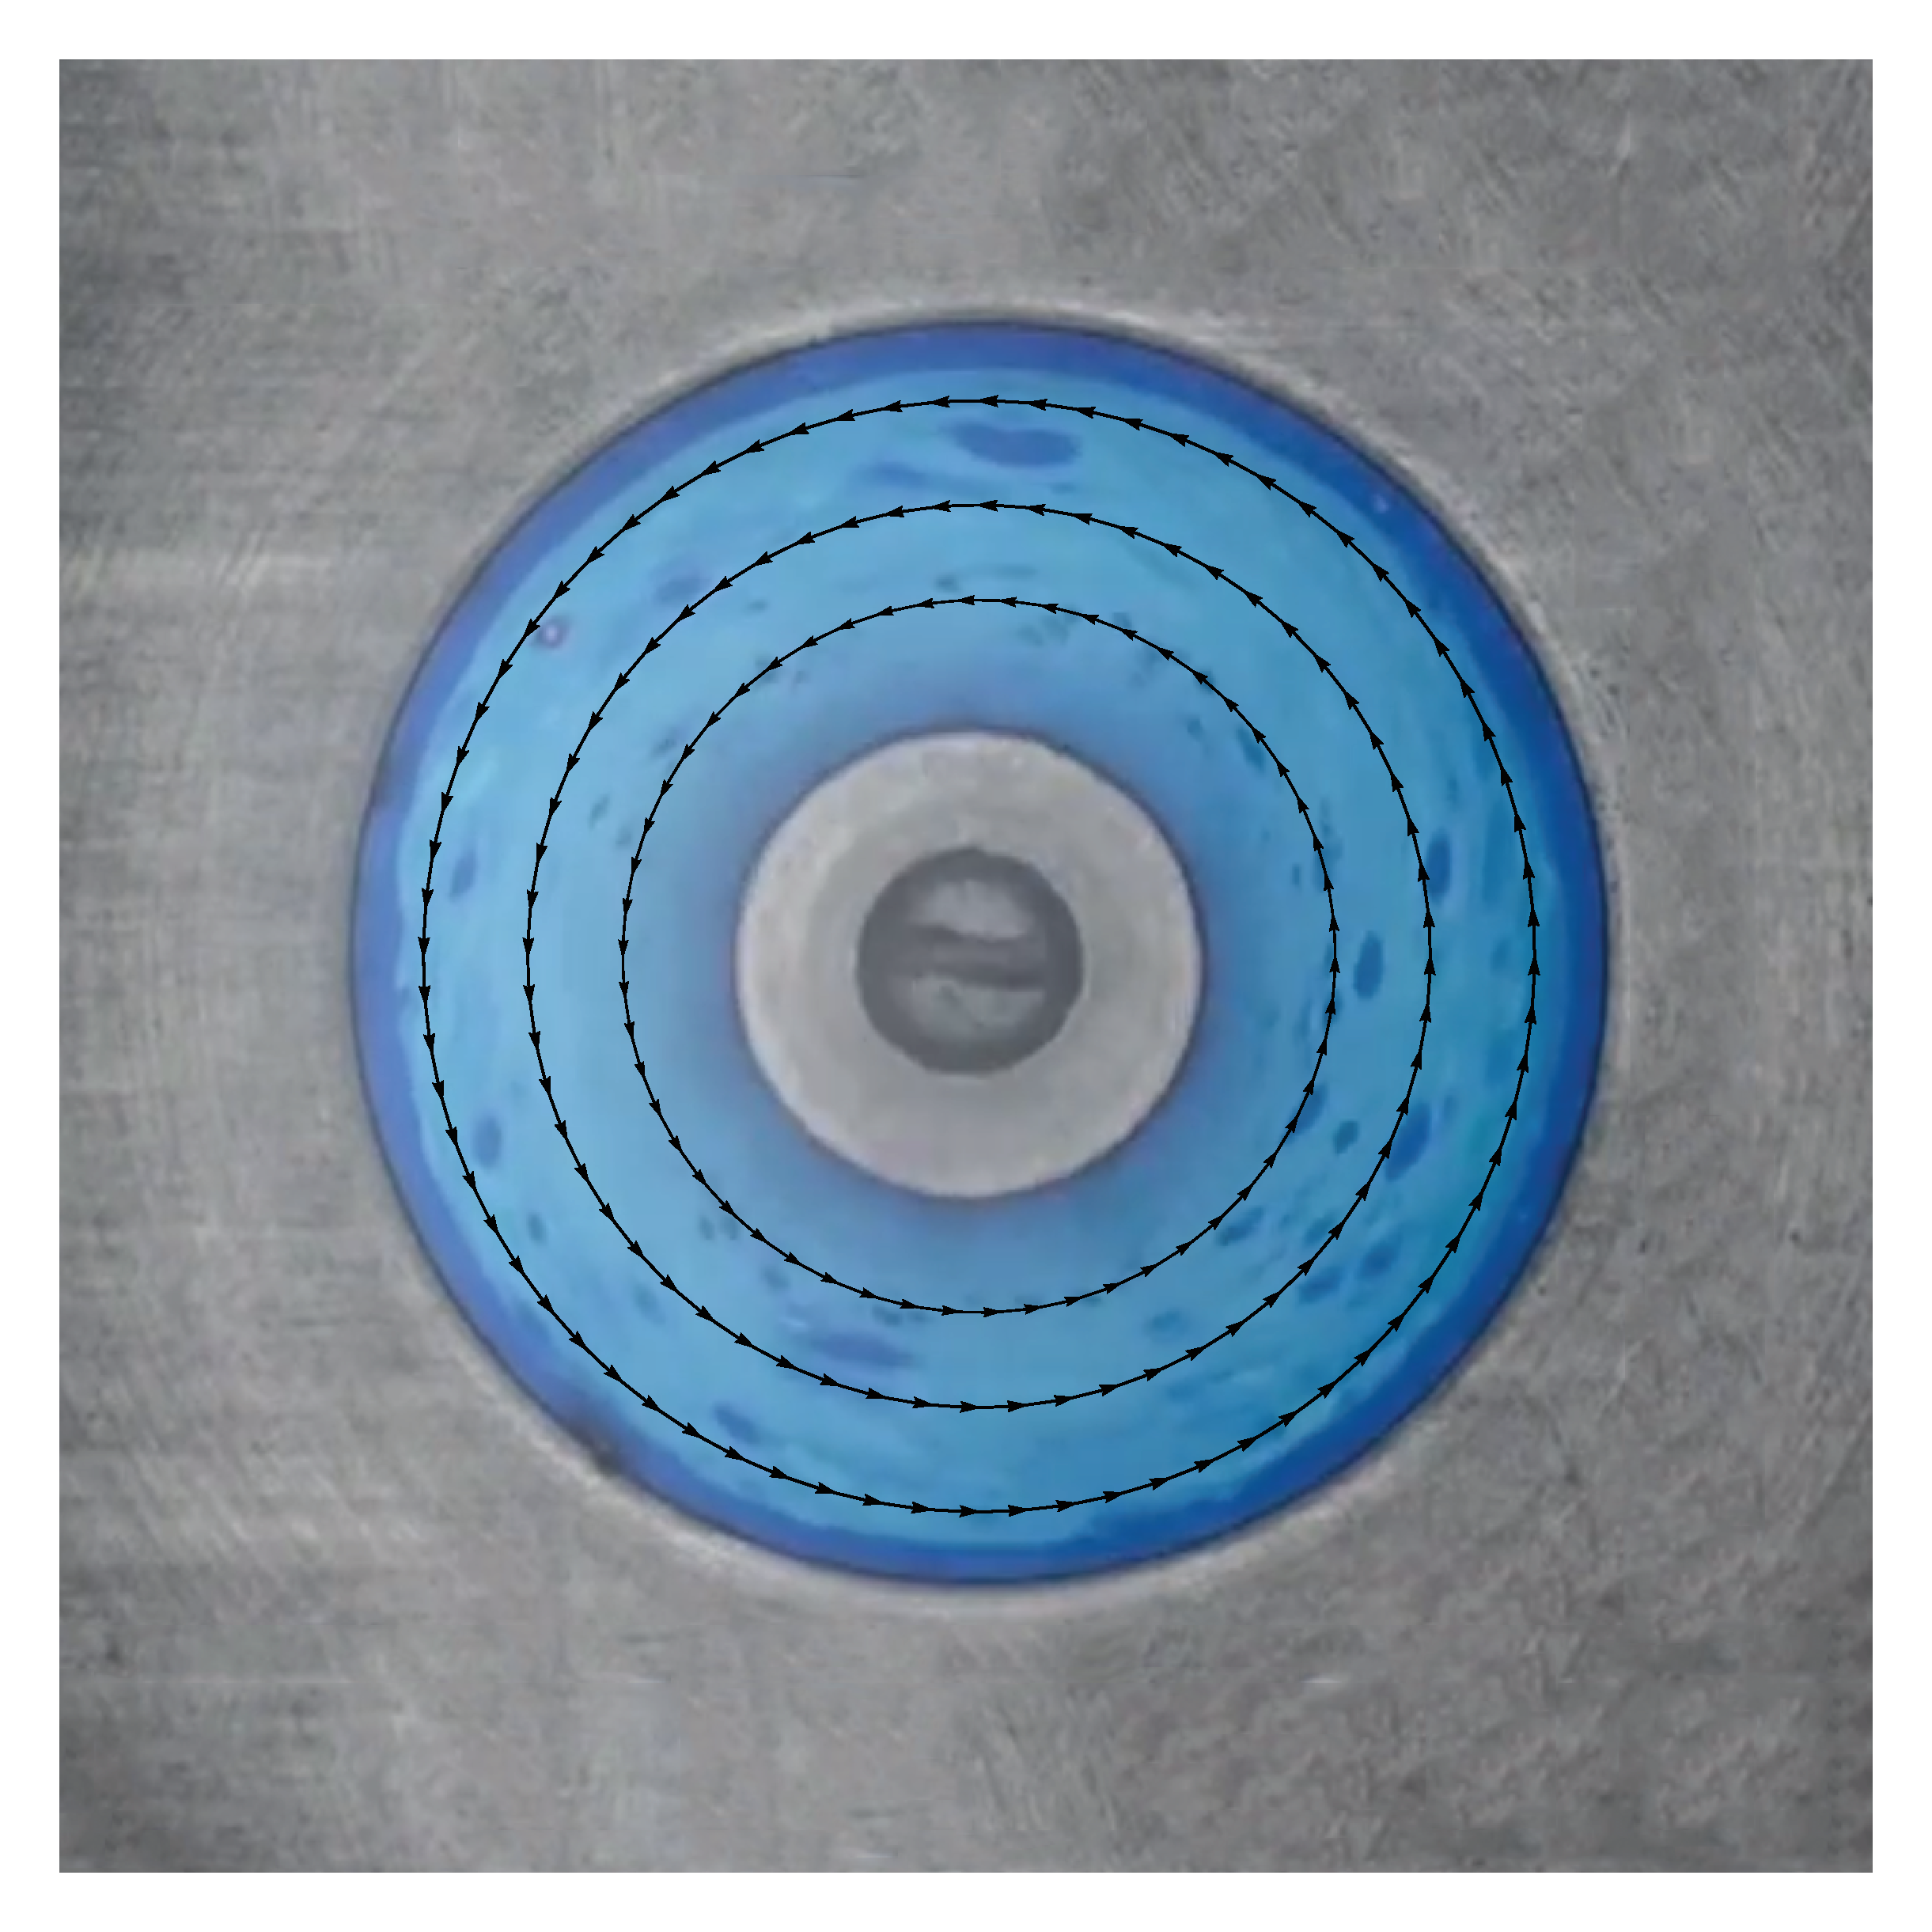
\includegraphics[width= .45\textwidth]{./figures/Pictures/physical_experiment_axi}}
\subfigure{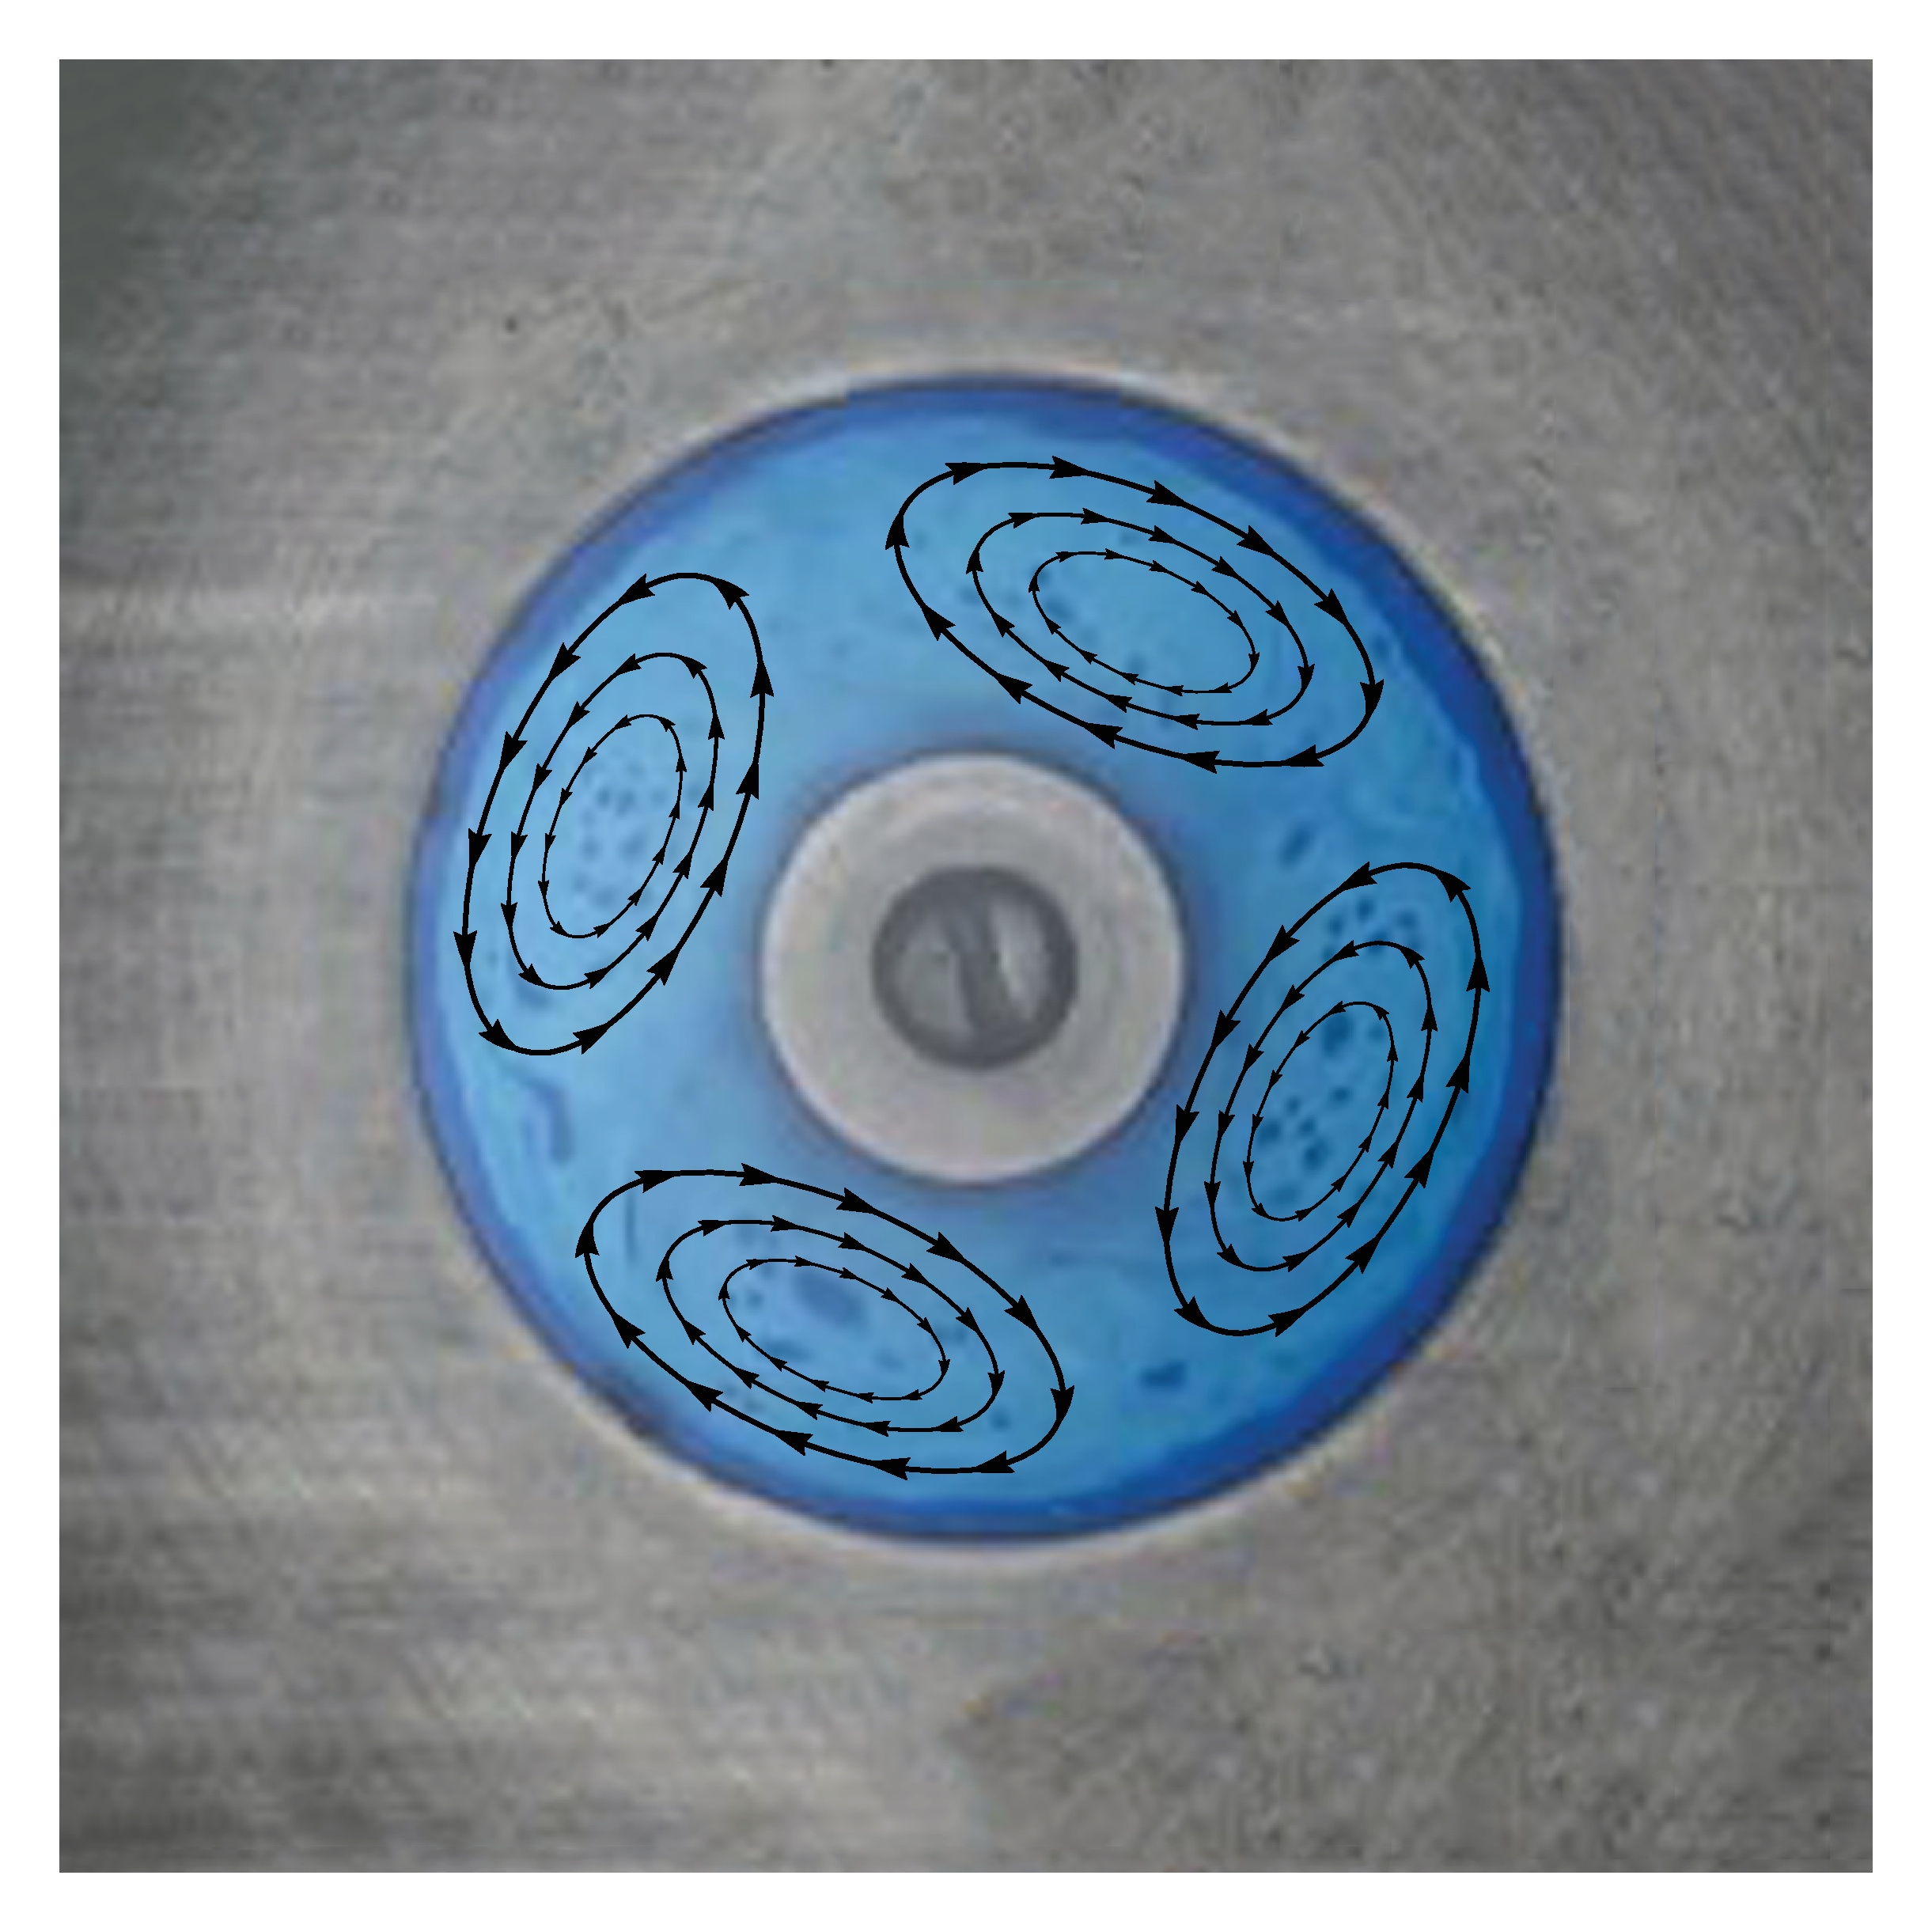
\includegraphics[width=.45\textwidth]{./figures/Pictures/physical_experiment_rotating}}
\caption{Snapshot of the two states that the flow exhibits in the physical experiment as the voltage is gradually increased between the boundaries, axisymmetric flow (left) and rotating wave flow (right). The axisymmetric flow is independent in time but the rotating wave pattern as shown in the snapshot rotates with respect to the boundaries; picture is adapted from \url{https://www.youtube.com/watch?v=WK5jRHR6NIg}. }\label{fig_exp_snap}
%[Snapshot of the axisymmetric and rotating waves flow in the physical experiment]
\end{center}
\end{figure}

As the applied voltage is incremented and then decremented in a small steps, $100$ current measurements spaced by $25$\ ms are performed and the average values of these measurements are used to calculate the Nusselt number $\mathrm{Nu}$, which is a dimensionless parameter defined as the ratio of total current to the conductive current. An Analysis of the data identified the critical voltage $V_c$ to be close to $40$ volts; at $V_c$, a primary transition from conduction to convection occurs. At $V < V_c$, the fluid flow is steady and charge was carried by ohmic conduction. For small $V>V_c$, the film flows in a series of counter-rotating pairs of laminar vortices. At $V\sim 200$ volts, a secondary transition was identified due to a sudden jump in the current fluctuations. At even higher voltages $V \gtrsim 600$ volts, the flow becomes turbulent.

This experiment has been repeated for different constant angular speeds of the inner electrodes to investigate the effect of the rotation on the primary transition. It is shown in~\cite{BAEWIS,AEWSDaDe}, that the primary transition is supercritical for different rotation rates, i.e. the amplitude of the convective vortices grow monotonically from zero. Furthermore, the rotation acts as a stabilizer of the flow, delaying the onset of convection.
These transitions can be reproduced with the numerical simulations of the mathematical model which we describe next.
%The limitations of the physical experimentation lead to another approach, that is, studying a mathematical model that copy the experiment.

\section{The Mathematical Model}\label{sec_mat_mod}
For the model, we assume that the film is confined between two concentric annular electrodes as shown in Figure~\ref{experiment_diagram}. An electric potential difference is applied between the boundaries with the inner electrode rotating at a constant angular speed. This section discusses the mathematical model describing the physical experiment and the base state solution of the governing equations. A brief overview of the pseudo-spectral numerical method, used to solve the perturbation equations from the base state, is also discussed.

\begin{figure}[t]
\centering{\includegraphics[width = .45\textwidth]{./figures/Pictures/ele_con_pic1}}
\caption{Relevant geometry of sheared annular electroconvection.}
\label{experiment_diagram}
%[Illustration of the experiment of annular electroconvection]
\end{figure}

\subsection{The governing equations}\label{sec_gov_equ}
In this section, the governing equations and the boundary conditions that model the experiment of annular electroconvection are presented. In the physical experiment, the thin film is confined in an annular region defined in cylindrical coordinates as, $r_i\le r\le r_o$. The film is a liquid crystal in Smectic~A phase with thickness $s$,  much smaller than the gap width $d = r_o-r_i,$ such that $d\gg s$. Considering this and the property of Smectic~A phase that inhibits motion between layers, we assume that the film can be considered as a 2D electrically conducting Newtonian fluid in the plane $z=0$. The density, viscosity and conductivity of the fluid are denoted by $\rho, \eta$ and $\sigma$ respectively. The inner electrode, $0\le r\le r_i$, is rotating at a constant angular speed $\omega_i$ and is held at an electric potential $V$. The outer electrode, $ r\ge r_o$, is held at zero potential and does not rotate. The conservation of momentum and the conservation of matter, given by the incompressible Navier-Stokes equations with an electric body force $q\mathbf{E}$, model the velocity field $\mathbf{u}(r,\theta,t) = u(r,\theta,t) \hat{\mathbf{r}} + v(r,\theta,t) \boldsymbol{\hat{\theta}}$
\begin{subequations}
\begin{align}
\label{Nav_Sto}
&\rho\left(\pderiv[]{\mathbf{u}}{t} + \left(\mathbf{u}\cdot\nabla\right)\mathbf{u}\right) = -\nabla P + \eta\nabla^2\mathbf{u} + q\mathbf{E},\\
\label{Incompress}
&\nabla\cdot\mathbf{u} = 0,
\end{align}
where $\hat{\mathbf{r}}$ is the unit vector in the radial direction, $\boldsymbol{\hat{\theta}}$ is the unit vector in the azimuthal direction, $\nabla$ is the 2D gradient operator, $P$ is the pressure,  $q$ is the surface charge density, $\mathbf{E} = -\left(\nabla\psi\right)|_{z=0}$ is the electric field in the film plane $z = 0$ and $\psi$ is the 3D electric potential.  The conservation of charge is expressed by the continuity equation
\begin{align}
\label{charge_con}
\pd{q}{t} = -\nabla\cdot \mathbf{J}, \hspace{1cm} \mathbf{J} = \sigma\mathbf{E} + q\mathbf{u},
\end{align}
where the current density $\mathbf{J}$ is composed of a term due to ohmic conduction density $\sigma\mathbf{E}$ and a term due to the fluid convection $q\mathbf{u}$. The electric potential $\psi$ satisfies the Laplace equation
\begin{align}
\label{laplace_eq}
\lb \nabla^2 + \pderiv[2]{}{z}\rb\psi = 0,
\end{align}
in the charge free region $z\ne 0$. To find the charge in the film region $z =0$, we note that by assuming that any magnetic effects are neglected, the 2D surface charge density $q$ satisfies Maxwell's equation~\cite{linearstability}
\begin{align}
\label{Maxwell_relation}
q = -2\epsilon_0 \pderiv{\psi}{z}\Big{|}_{z=0^+},
\end{align}
where $\epsilon_0$ is the permittivity of free space.
\end{subequations}
%The Maxwell's equation is presented by  which describes a nonlocal relation between the surface charge density and the 3D electric potential $\psi$. Therefore, in the space $z\ne0$, that is free of charge, the 3D electric potential satisfy Laplace equation,
%\begin{align}
%\label{laplace_eq}
%\lb \nabla^2 + \pderiv[2]{}{z}\rb\psi = 0.
%\end{align}

Equation ~(\ref{Nav_Sto})--(\ref{Maxwell_relation}) are subject to the following boundary conditions.
The velocity field satisfies no-slip boundary conditions
\begin{subequations}
\begin{align}
&\mathbf{u} = \omega_i r_i \boldsymbol{\hat{\theta}}, &  & r = r_i,\\
&\mathbf{u} = 0, & & r = r_o,
\end{align}
at each electrode.
The potential $\psi$ is set to zero at infinity
\begin{align}
\lim_{z \to \pm \infty} \psi(r,\theta,z) = 0,
\end{align}
and, at $z = 0$, takes on the imposed voltage, so that
 \begin{equation}
    \psi(r,\theta,0)= \psi_2(r,\theta) =
\begin{cases}
    V,& \text{for } r \le r_i,\\
    0,              & \text{for } r\ge r_o,
\end{cases}
\end{equation}
\end{subequations}
where $\psi_2$ is the 2D electric potential in the fluid plane.

A streamfunction-vorticity formulation can be used to eliminate the pressure term, where the fluid velocity field is replaced by two scalar function $\omega$ and $\phi$ defined as follows
\begin{align}
\label{stream}
\mathbf{u} &= \nabla\phi\times\hat{\mathbf{z}}, & \nabla\times\mathbf{u} &= \omega\hat{\mathbf{z}},
\end{align}
where $\omega = \omega(r,\theta,t)$ and $\phi = \phi(r,\theta,t)$ are the vorticity and streamfunction of the flow, respectively. In addition, we can define a characteristic length, time and charge. If we let the imposed voltage $V$ denote a representative voltage over a length scale of size $d = r_o - r_i$ and a relaxation time $\tau_c = \epsilon_0 d/\sigma$, where $\sigma$ is the conductivity and $\epsilon_0$ is the permeability constant, then we obtain the following natural nondimensionalization
\begin{align}
\label{nondimes}
r &= d \tilde{r},     & \phi &= \frac{\sigma d}{\epsilon_0}\tilde\phi, &  \psi &= V\tilde{\psi} & t &= \tau_c\tilde{t}, & q & = \frac{\epsilon_0 V}{d}\tilde{q},
\end{align}
where the tilde represents the dimensionless variables.
Applying the formulation~(\ref{stream}) to~(\ref{Nav_Sto})--(\ref{Maxwell_relation}), nondimensionalizing with~(\ref{nondimes}) and dropping the tilde, we obtain the system of equations describing the evolution of the dimensionless physical quantities, vorticity $\omega$, streamfunction $\phi$, charge density $q$, the 2D potential in the fluid $\psi_2$ and the 3D potential $\psi$,
\begin{subequations}
\begin{align}
\label{dim_less_1}
&\nabla^2\phi = -\omega, \\
\label{dim_less_2}
&\pd{\omega}{t}+\lb \mathbf{u}\cdot\nabla\rb\omega =\mathcal{P}\nabla^2\omega + \mathcal{PR}\lb \nabla\psi_2\times\nabla q\rb\cdot\mathbf{\hat{z}},\\
&\pd{q}{t}+\lb \mathbf{u}\cdot\nabla\rb q = \nabla^2\psi_2,\\
&\lb \nabla^2 + \pderiv[2]{}{z}\rb\psi = 0, \hspace{2cm} q = -2\pd{\psi}{z}\Big{|}_{z=0^+}, \label{dim_less_end}
\end{align}
\end{subequations}
where the nondimensional parameter groups are the Rayleigh number $\mathcal{R}$ and the Prandlt number $\mathcal{P}$ defined as
\begin{align}
 \mathcal{R} &= \frac{\epsilon_{0}^2V^2}{\sigma\eta}, & \mathcal{P} &= \frac{\epsilon_{0}\eta}{\rho\sigma d},
\end{align}
respectively.
The Rayleigh number $\mathcal{R}$, which is proportional to the square of the applied voltage $V$, describes the relative strength of the applied electric forcing to the viscous dissipation, and the Prandlt number $\mathcal{P}$ is a fluid parameter that describes the ratio of the charge relaxation time to the viscous relaxation time.

The boundary conditions also transform and become
\begin{subequations}
\begin{align}
\label{bcd_1}
&\pderiv[]{}{r}\phi(r_o,\theta)= 0, &  &\pderiv[]{}{\theta}\phi(r_o,\theta) = 0,\\
&\pderiv[]{}{r}\phi(r_i,\theta)= -\frac{\omega r_i \epsilon_0}{\sigma} = -\omega_i r_i \tau_c,& &\pderiv[]{}{\theta}\phi(r_i,\theta) = 0,\\
& \psi_2(r_i,\theta) = 1,    &    &\psi_2(r_o,\theta) = 0,
\end{align}
\begin{equation}
    \psi(r,\theta,0)=
\begin{cases}
    1,& \text{for } 0\le r \le r_i,\\
    \psi_2(r,\theta), & \text{for } r_i\le r \le r_o,\\
    0,              & \text{for } r\ge r_o,
\end{cases}
\end{equation}
\begin{equation}
\label{bc_dim_end}
\lim_{z \to \pm \infty} \psi(r,\theta,z) = 0,
\end{equation}
\end{subequations}
where $r_i, r_o$ are dimensionless quantities scaled by $d$ and the the tilde have once again been dropped for clarity.
The cross width of the film in dimensionless units is then, $r_o-r_i = 1$, where $r_o$ is the dimensionless radius of the outer electrode set at zero electric potential and $r_i$ is the dimensionless radius of the inner electrode set at an electric potential of 1. It is convenient to express the radii of the annular geometry with the aspect ratio $\alpha = r_i/r_o$. Introducing this, the dimensionless radii can be express as
\begin{align}
\label{aspect_ratio}
r_{i} & = \frac{\alpha}{1- \alpha}, &  r_o & = \frac{1}{1- \alpha}.
\end{align}

Equations~(\ref{dim_less_1})--(\ref{dim_less_end}) with the boundary conditions~(\ref{bcd_1})--(\ref{bc_dim_end}) describe the sheared annular electroconvection of any arrangement of 2D thin conductive film freely suspended in empty space. In other words, the model still holds for the unsheared electroconvection with appropriate changes to the boundary conditions.


\subsection{The perturbation equations}
The governing equations introduced in the previous section are now solved for the case of sheared annular electroconvection. Cylindrical coordinates $(r,\theta,z)$ are employed, where $z = 0$ is defined to be the plane in which the film is suspended between the two circular electrodes.
At very low rotation rates, an axisymmetric flow is observed. We call this flow the base state and denote it by a superscript zero. This flow can be computed analytically as follows.
With the rotation of the inner electrode generating a steady Couette shear described by the dimensionless Reynolds number
\begin{align}
\mathrm{Re} = \frac{r_i\Omega}{\mathcal{P}},
\end{align}
where $\Omega = \tau_{c}\omega_i$ is the dimensionless angular frequency of the inner electrode,
 the radial derivative of the base state streamfunction and the vorticity~\cite{EDCTAFUCF} can be obtained from
%The rotation of the inner electrodes generates a Couette shear in the base state that we denote with a superscript zero. The base state of the streamfunction and the vorticity given an imposed shear is obtained by,
\begin{align}
\label{base_phi}
\pderiv[]{\phi^{(0)}(r)}{r} &= \frac{\alpha^2\Omega}{1-\alpha^2}\left( r-\frac{1}{r(1-\alpha)^2}\right),\\
%\end{align}
%\begin{align}
\label{base_omega}
 \omega^{0}(r) &= 0.
\end{align}
The base state of the charge density and the potential can also be solved analytically and one can verify that
\begin{align}
\label{base_q}
q^{(0)}(r) = \frac{2}{\ln{\alpha}}\left( \frac{1}{r}F\left(\frac{1}{2},\frac{1}{2};1;\frac{r_o^2}{r^2}\right) - \frac{1}{r_i}F\left(\frac{1}{2},\frac{1}{2};1;\frac{r^2}{r_i^2}\right)\right)
\end{align}
\begin{equation}
\label{base_psi2}
    \psi_2^{(0)}(r)=
\begin{cases}
    1,& \text{for } 0\le r \le r_i,\\
    \frac{1}{\ln{\alpha}}\left(\ln{(1-\alpha)} + \ln{r}\right), & \text{for } r_i\le r \le r_o,\\
    0,              & \text{for } r\ge r_o,
\end{cases}
\end{equation}
\begin{equation}
\label{base_psi}
\psi^{(0)}(r,z) = \int_0^\infty A(k)J_0(kr)e^{-kz} \text{d}k
\end{equation}
where $F$ is a hypergeometric function~\cite{EDCTAFUCF}, $J_0$ is the zeroth Bessel function and
\begin{align}
A(k) = k\int_0^\infty \psi^{(0)}(r,0)J_0(kr)r\text{d}r.
\end{align}
We note that, in this experiment, the inner electrodes is rotating at a constant rate while the outer electrodes is fixed.  However, independent rotations of the electrodes can be dealt by applying a transformation to a rotating frame of reference, where the outer electrode is stationary. The Coriolis forces introduced by the transformation can be absorbed into the pressure term of~(\ref{Nav_Sto}).

We can now decompose the solutions into this base state (axisymmetric) component denoted by a superscript zero and a perturbation from the base state denoted by a superscript one so that
\begin{subequations}
\begin{align}
\phi(r,\theta,t)   = \phi^{(0)}(r)   &+ \phi^{(1)}(r,\theta,t),\\
\omega(r,\theta,t) = \omega^{(0)}(r) &+ \omega^{(1)}(r,\theta,t),\\
q(r,\theta,t)      = q^{(0)}(r)      &+ q^{(1)}(r,\theta,t),\\
\psi_2(r,\theta,t) = \psi_2^{(0)}(r) &+ \psi_2^{(1)}(r,\theta,t),\\
\psi(r,\theta,z,t) = \psi^{(0)}(r,z) &+ \psi^{(1)}(r,\theta,z,t).
\end{align}
\end{subequations}
Upon applying the decomposition of the solution into a base state and perturbation from the base state and substituting in~(\ref{dim_less_1})--(\ref{dim_less_end}), we obtain the following set of equations
\begin{subequations}
\begin{align}
\label{pert_1} &\nabla^2 \phi^{(1)} = -\omega^{(1)},\\
&\pderiv[]{q^{(1)}}{t} + \mathcal{J}_{(q,\phi)} - \nabla^2\psi_2^{(1)} = 0, \\
&\pderiv[]{\omega^{(1)}}{t} + \mathcal{J_{(\omega,\phi)}} = \mathcal{P} \nabla^2\omega^{(1)} + \mathcal{PR}\mathcal{J}_{(\psi_2,q)},\\
\label{pert_end} &\left(\nabla^2_{r\theta} + \pderiv[2]{}{z} \right)\psi^{(1)} = 0, \hspace{2cm}
q^{(1)} = -2\pderiv[]{\psi^{(1)}}{z}\Big{|}_{z=0},
\end{align}
\end{subequations}
where $\mathcal{J}_{(i,j)}$ are the nonlinear Jacobian terms
\begin{subequations}
\begin{equation}
\label{Jacobian_1}
\mathcal{J}_{(q,\phi)} = \frac{1}{r}\left(\pderiv[]{q^{(0)}}{r}\pderiv[]{\phi^{(1)}}{\theta} + \pderiv[]{q^{(1)}}{r}\pderiv[]{\phi^{(1)}}{\theta}
                                       -  \pderiv[]{\phi^{(0)}}{r}\pderiv[]{q^{(1)}}{\theta} - \pderiv[]{\phi^{(1)}}{r}\pderiv[]{q^{(1)}}{\theta}   \right),
\end{equation}
\begin{equation}
\mathcal{J}_{(\omega,\phi)} = \frac{1}{r}\left(\pderiv[]{\omega^{(0)}}{r}\pderiv[]{\phi^{(1)}}{\theta}+\pderiv[]{\omega^{(1)}}{r}\pderiv[]{\phi^{(1)}}{\theta}
                                       -  \pderiv[]{\phi^{(0)}}{r}\pderiv[]{\omega^{(1)}}{\theta} - \pderiv[]{\phi^{(1)}}{r}\pderiv[]{\omega^{(1)}}{\theta}   \right),
\end{equation}
\begin{equation}
\mathcal{J}_{(\psi_2,q)} = \frac{1}{r}\left(\pderiv[]{\psi_2^{(0)}}{r}\pderiv[]{q^{(1)}}{\theta} - \label{Jacobian_end}
\pderiv[]{q^{(0)}}{r}\pderiv[]{\psi_2^{(1)}}{\theta}
                                        + \pderiv[]{\psi_2^{(1)}}{r}\pderiv[]{q^{(1)}}{\theta} - \pderiv[]{q^{(1)}}{r}\pderiv[]{\psi_2^{(1)}}{\theta} \right).
\end{equation}
\end{subequations}
The perturbation variables $\phi^{(1)},\psi_2^{(1)}$ and $\psi^{(1)}$ must satisfy the following boundary conditions
\begin{subequations}
\begin{equation}
\phi^{(1)}(r_i,\theta) = \pderiv[]{}{r}\phi^{(1)}(r_i,\theta) =
\phi^{(1)}(r_o,\theta) = \pderiv[]{}{r}\phi^{(1)}(r_o,\theta) = 0,
\end{equation}
\begin{equation}
\psi_2^{(1)}(r_i,\theta) = \psi_2^{(1)}(r_o,\theta) = 0,
\end{equation}
\begin{equation}
    \psi^{(1)}(r,\theta,0)=
\begin{cases}
    0,& \text{for } 0\le r \le r_i,\\
    \psi_2^{(1)}(r,\theta), & \text{for } r_i\le r \le r_o,\\
    0,& \text{for } r \ge r_o,
\end{cases}
\end{equation}
\begin{equation}
\lim_{z \to \pm \infty} \psi^{(1)}(r,\theta,z) = 0.
\end{equation}
\end{subequations}
This latter set of equations determines the perturbation from the base state and its numerical solution will be considered in the subsequent sections.

\section{The Numerical Solver}\label{sec_num_sol}
In this section, we provide a brief overview of the numerical time stepper implemented in MATLAB~\cite{PeiChunTsain} that we will use for our numerical bifurcation method. The solutions of~(\ref{dim_less_1})--(\ref{dim_less_end}) are approximated with a pseudospectral method in order to take advantage of the efficiency of the Fast Fourier Transform (FFT) and the inherent convergence properties of this method~\cite{Trefethen}.
The periodic boundary conditions suggest the choice of the Fourier basis $\{e^{im\theta}\}$ in the angular coordinate and, due to the no-slip condition which leads to steep changes at the boundaries, the choice of Tchebychev basis for the radial coordinate becomes favorable to avoid Gibbs phenomenon. Thus, the 2D physical quantities, the streamfunction $\phi$, the vorticity $\omega$, the charge density $q$ and the electric potential $\psi_2$, can be approximated using a truncated Fourier series $\{e^{im\theta}\}$ in the $\boldsymbol{\hat{\theta}}$ direction and a series of Tchebychev polynomials $T_n(r)$ in the $\hat{\mathbf{r}}$ direction, that is
\begin{subequations}
\begin{align}
\phi^{(1)}(r,\theta,t) &= \sum_{n=0}^{N_c}\sum_{m = -K}^{K}\tilde{\phi}_{nm}(t)e^{im\theta}\,T_n(x),\\
\omega^{(1)}(r,\theta,t) &= \sum_{n=0}^{N_c}\sum_{m = -K}^{K}\tilde{\omega}_{nm}(t)e^{im\theta}\,T_n(x),\\
q^{(1)}(r,\theta,t) &= \sum_{n=0}^{N_c}\sum_{m = -K}^{K}\tilde{q}_{nm}(t)e^{im\theta}\,T_n(x),\\
\psi_2^{(1)}(r,\theta,t) &= \sum_{n=0}^{N_c}\sum_{m = -K}^{K}\tilde{\psi_2}_{nm}(t)e^{im\theta}\,T_n(x),
\end{align}
\end{subequations}
where $K$ is the highest Fourier mode, $N_c$ is the order of the highest Tchebychev polynomial and
\begin{align}
x = 2r - \frac{1+\alpha}{1-\alpha},
\end{align}
linearly maps $r \in \left[\frac{\alpha}{1-\alpha}, \frac{1}{1-\alpha}\right]$ to $x \in [-1,1]$ that spans the film. The reason for this remapping is to utilize the collocation points, $x_j = \cos(\pi j/N_c),\ j = 0,1,\ldots,N_c$, at which the collocation method that approximates the solution as a truncated Tchebychev polynomial series  makes the residual equal to zero.

The time-stepping was implemented in two different schemes. The first scheme is an implicit-explicit Euler method in which the linear terms are computed implicitly and the nonlinear terms are computed explicitly. Using this scheme, the time derivative is approximated as
\begin{equation}
\label{scheme_euler}
\pderiv[]{u}{t}  \approx \frac{u^{(k+1)} - u^{(k)}}{\delta t}.
\end{equation}
where $\delta t$ is a prescribed time step and $u$ is the discretized solution vector. The other scheme that is implemented uses a second-order implicit backward difference method (BDI2) in which the time derivative is approximated as
\begin{equation}
\label{BDI2}
\pderiv[]{u}{t} \approx \frac{3u^{(k+1)} -4u^{(k)}+ u^{(k-1)}}{2\delta t},
\end{equation}
and the nonlinear terms given by equations~(\ref{Jacobian_1})--(\ref{Jacobian_end}) are approximated using a first-order Adams-Bashforth method (AB$_1$).

The numerical time-stepper for the smectic electroconvection is complicated by a nonstandard boundary condition. The surface charge $q$ is not only coupled to flow motion, but also regulated by the 2D electric potential field $\psi_2$. To handle this situation, a different approach is required to resolve the nonlocal coupled electric body force that involves Maxwell's equation~(\ref{pert_end}) which connects the charge density with the electric potential. However, the nonlocal calculation of the 3D potential and the charge field are assumed to couple instantaneously and therefore do not involve any time derivatives. The Laplace equation is solved implicitly in integral form where the boundary condition is resolved by decomposing the field using a pseudospectral technique~\cite{PeiChunTsain}.

With the proper initial conditions, boundary conditions and time step, the 2D electric potential $\psi_2$ is computed simultaneously with the surface charge $q$ by means of the nonlocal mapping. The vorticity $\omega$ can then be obtained from the computed $q$ and $\psi_2$ leading to the computation of the streamfunction $\phi$. The Orszag 3/2 aliasing rule is performed when dealing with the nonlinear terms.

The two different time-stepping were used to estimate and compare the accuracy of the solutions. It was found that both implementations yield in consistent simulation results in the weakly nonlinear regime and the second scheme (AB$_1$)/(BDI2) gives second order accuracy~\cite{PeiChunTsain}. For high Rayleigh number, the second scheme was more stable and preferable where the time step $\delta t$ is limited due to computational instability. For our implementation, we use the second scheme.

The time stepper computes some extra integrated physical quantities such as a dimensionless  Nusselt number $\mathrm{Nu}$ and a mean area density of the kinetic energy. The Nusselt number is defined as  the ratio of total current to the conductive current transported by diffusion process. For more detailed explanation of the time stepper, the reader is referred to~\cite{PeiChunTsain}.

\subsection{Numerical results}
For comparative purposes with the latter part of this thesis, we highlight in this section some of the numerical results obtained in~\cite{PeiChunTsain,DNSSAE}. As in this thesis, the main control parameter of interest is the Rayleigh number $\mathcal{R}$. Long time integrations of a random initial condition are performed to study the effect of the Rayleigh number $\mathcal{R}$ on the base state solution, while fixing the other nondimensional parameters $\mathcal{P},\mathrm{Re}$ and $\alpha$. The flow undergoes a primary transition from axisymmetric to rotating waves as $\mathcal{R} > \mathcal{R}_c$. This transition is found to be a supercritical Hopf bifurcation for a wide range of dimensionless parameters $\{\mathcal{P},\alpha,\mathrm{Re}\}$. Amplitude vacillating waves are observed for higher values of $\mathcal{R}$. Further increases in $\mathcal{R}$ cause the flow to exhibit a steady convective wave state with a different integer number of vortices distinct in character from the primary transition and the flow eventually becomes turbulent for relatively large Rayleigh numbers.

The effect of the aspect ratio $\alpha$, the Prandlt number $\mathcal{P}$ and the Reynolds number $\mathrm{Re}$ on the primary transition are also investigated in~\cite{PeiChunTsain}. In particular, the critical Rayleigh number $\mathcal{R}_c$ and the critical mode $m_c$, (the number of counter rotating waves pairs) are observed for various values of these parameters. The authors find that, the aspect ratio $\alpha$ strongly influences $\mathcal{R}_c$ and $m_c$, with numerous codimension-two points observed when two critical modes $m = m_c$ and $m=m_c + 1$ become unstable. Eventually one mode saturates to a convective state and the other slowly decays.
Changes in the Prandlt number $\mathcal{P}$, which is a fluid parameter that describes the relation between the charge relaxation time and the viscous relaxation, are found to  effect the nonlinear advection terms compared to the viscous and external driven forces which can also be analyzed from~(\ref{dim_less_2}).
The Reynolds number $\mathrm{Re}$ which describes the imposed shear, is found to suppress the onset of convection as the shear is increased. It is also found that a decreasing trend in the unstable mode $m_c$ as the applied shear is increased. In other words, an increase of applied shear decreases the number of paired vortices in the flow.

\chapter{Continuation Methods}\label{ch_cm}
Continuation methods are powerful tools that can be used to find solutions of a parameterized nonlinear system of equations of the form
\begin{align} \label{non_sys}
&\mathbf{G}(\mathbf{x},\alpha) = 0,& & \mathbf{G}: \mathbb{R}^n\times\mathbb{R}^p\rightarrow\mathbb{R}^{n},
\end{align}
where $\mathbf{x} \in \mathbb{R}^{n}$ is a discretized solution of the nonlinear system of $n$-equations and
$\alpha \in \mathbb{R}^p$ are parameters of the system. The solutions  of the nonlinear system of equations~(\ref{non_sys}) are manifolds connected at \emph{singularity} solutions or bifurcation points. In the case of  $p =1$, these manifolds are curves $\Gamma$ that lie in the space $(\mathbf{x},\alpha)$. In practice, such curves are approximated by a set of discrete points $\left\{(\mathbf{x}_i,\alpha_i)\right\}_{i=0}^n$ which correspond to an approximate solutions of the nonlinear system~(\ref{non_sys}), and which can be found using continuation methods. Specifically, assume that an approximate solution $\mathbf{x}_0$ for the nonlinear system~(\ref{non_sys}) is known for parameter value $\alpha = \alpha_0$ i.e. $(\mathbf{x}_0,\alpha_0)$ is a point on $\Gamma$. This point is used to find the next point $(\mathbf{x}_1,\alpha_1)$  on the curve and this new point to find the next, and so on, thus tracing out the curve.

This chapter gives an overview of continuation methods and their application to dynamical systems. In Section~\ref{sc_ti_ap}, we discuss matrix-free methods which are memory-efficient methods that are effective for the application of continuation methods to large-dimensional systems. The application of these methods to detect equilibria and periodic solutions and to identify their local behaviours for the annular electroconvection problem are discussed in Section~\ref{sc_ti_ap} and~\ref{sec_lin_sta_ana}.

\section{Methodology}\label{sc_meth}
In general, continuation methods consist of a two step, predictor-corrector procedure. In the first step a guess $(\hat{\mathbf{x}}_1,\hat{\alpha}_1)$ is predicted by an extrapolation from a known solution $(\mathbf{x}_0,\alpha_0)$ to the nonlinear system~(\ref{non_sys}). In the second step, a nonlinear solver, e.g. of Newton type, is used to correct the guess to within a desired tolerance.

The most common continuation method in the literature is pseudo-arclength continuation~\cite{Con_meth_2,Con_meth_1}, which was introduced by Keller~\cite{Keller} in the late 1970s. In pseudo-arclength continuation, the solution curves $\Gamma$, the state variable $\mathbf{x}$, and a scalar parameter of the nonlinear system $\alpha$ are parameterized using an independent arclength parameter $s$, i.e. $\Gamma(s):= (\mathbf{x}(s),\alpha(s))$. Using this approach, the solution curves are traced out along the arclength parameter $s$. In one type of pseudo-arclength continuation known as the \emph{Keller method}, the nonlinear solver makes the correction along the plane orthogonal to the tangent space of the curve~\cite{Con_meth_1}. This method is desirable for its ability to trace curves that fold back on themselves. At these \emph{fold} points (see Figure~\ref{fig_con_non_sys}), the Jacobian of the nonlinear system~(\ref{non_sys}) with respect to $\mathbf{x}$  becomes singular, leading to problems in the solutions of the linear system obtained using Newton-like solvers which depend mainly on the Jacobian to approximate solutions of~(\ref{non_sys}). For the sheared annular electroconvection problem, we do not anticipate \emph{fold} points. Thus, we choose to implement natural numerical continuation methods in which the solution curves $\Gamma$ are parametrized using the natural parameter $\alpha$ of the nonlinear system, $\Gamma(\alpha):=\left(\mathbf{x}(\alpha),\alpha\right)$. This method makes the correction along the plane orthogonal to the paramater $\alpha$ plane (see Figure~\ref{fig_con_non_sys}), and thus fails at \emph{fold} points. The benefit of natural continuation is that it is slightly easier to implement then pseudo-arclength continuation.
\begin{figure}[t]
\centerline{\includegraphics[ width = 1.1\textwidth]{./figures/Pictures/Ill_Nat_CM.pdf}}
\caption{The natural continuation method with a secant extrapolation. The solution points on the curve are represented by $(\mathbf{x}_i,\alpha_i)$, the vertical axis represents some norm of the state vector $\mathbf{x}$ and the horizontal axis represents the parameter of the nonlinear system $\alpha$.}
\label{fig_con_non_sys}
%[Illustration of the natural continuation method with a secant extrapolation]
\end{figure}

The methodology of the natural continuation method  is illustrated in Figure~\ref{fig_con_non_sys}. In the first step, a guess $(\mathbf{x}_{i+1}^{(0)},\alpha_{i+1})$ is generated by an extrapolation  along a secant line from the previously computed solutions $(\mathbf{x}_{i},\alpha_{i})$ :
\begin{align}
& \alpha_{i+1} = \alpha_i + \delta,  && i \ge 0,\\
&\mathbf{x}_{i+1}^{(0)} = \mathbf{x}_{i},  && i = 0,     &&\\
&\mathbf{x}_{i+1}^{(0)} = \mathbf{x}_{i} + \frac{\mathbf{T}}{\|\mathbf{T}\|_2} \delta,  && i \geq 1,  && \mathbf{T} = \mathbf{x}_{i}-\mathbf{x}_{i-1}.
\end{align}
Here, the subscript $i$ denotes the point on the curve, the superscript denotes the number of nonlinear solver iterations and $\delta$ is a small increment step of the parameter $\alpha$.
In the second step, a Newton-Raphson solver can be used to refine the guess to within a given tolerance along the plane orthogonal to the axis of the parameter $\alpha$, i.e. for which $\alpha$ is constant. Specifically the iterate $\mathbf{x}_{i}^{(k+1)}$ can be found from the following linear equation
\begin{subequations}\begin{align}
\mathrm{D}_{\mathbf{x}}\mathbf{G}(\mathbf{x}_{i}^{(k)},\alpha_i)\delta \mathbf{x} &= -\mathbf{G}(\mathbf{x}_{i}^{(k)},\alpha_i),\\
\mathbf{x}_{i}^{(k+1)} &=\mathbf{x}_{i}^{(k)} + \delta \mathbf{x},
\end{align}\end{subequations}
where $\mathrm{D}_{\mathbf{x}}\mathbf{G}$ is the Jacobian of $\mathbf{G}$ with respect of $\mathbf{x}$ and $\delta{\mathbf{x}}$ is a Newton correction.
%Although the natural continuation methods is easier to implement than the pseudo-arclength, it fails to trace folds (see Figure~\ref{fig_con_non_sys}). At this fold points, the Jacobian of the nonlinear system $\mathrm{D}_{\mathbf{x}}\mathbf{G}(\mathbf{x},\alpha)$ becomes singular. In this case, pseudo-arclength continuation (see \cite{Con_meth_2}, \cite{Con_meth_1}), in which the nonlinear solver makes the correction along the plane orthogonal to the tangent space of the curve, is the appropriate choice. However, we do not anticipate folds, therefore we choose to implement a numerical natural continuation method.
%The solution points on the curve are represented by $\mathbf{X}_i = (\mathbf{x}_i,\alpha_i)$, the yaxis represents some norm of the state vector $\mathbf{x}$ and the xaxis represents the parameter of the nonlinear system $\alpha$.
%
%The pseudo-arclength methods have advantages on the natural continuation methods which fails to trace the solution curves around folds. In the pseudo-arc ince it traces the solution curves even around folds where the Jacobian of the nonlinear system becomes singular. In the pseudo-arclength, the
%%This type of parametrization is known as the natural parametrization.
%...
%We implement the numerical natural continuation method from scratch in MATLAB. We choose a secant extrapolation to predict the guess and Newton-Raphson nonlinear solver to correct the guess to the solution.
%%In the natural parametrization, the solution curve we denote $\Gamma$ is parametrized using the nonlinear system parameter $\alpha$.
%In the predictor step, starting from the known solution $(\mathbf{x}_0,\alpha_0)$, we choose the guess point $(\hat{\mathbf{x}}_1,\hat{\alpha}_1)$ such that,
%\begin{equation*}\begin{split}  \hat{\mathbf{x}}_1 = \mathbf{x}_0\\ \hat{\alpha}_1 = \alpha_0 + \delta, \end{split}\end{equation*} where $\delta$ is a step size, and then
\section{Application to Dynamical Systems}\label{sc_app}
One of the applications of continuation methods is to detect and compute invariant limit sets, such as steady states, limit cycles and invariant tori, of continuous dynamical systems of the form
\begin{align}
\label{dyn_sys}
&\deriv[]{}{t}\mathbf{u} = \mathbf{f}(\mathbf{u},\mu),& & \mathbf{f}: \mathbb{R}^n\times\mathbb{R}^p\rightarrow\mathbb{R}^n,
\end{align}
where $\mathbf{u}:=\mathbf{u}(t) \in \mathbb{R}^n$ is a state variable of the dynamical system and $\mu \in \mathbb{R}^p$ are the parameters of the system.  Upon obtaining these invariant limit sets, one can investigate their local behaviours, e.g. using linear stability analysis, and in the process, identify bifurcation points. The aim is to find representations (qualitative and quantitative) of the different types of behaviour that the system may exhibit depending on key parameters. The results can then be summarized in a bifurcation diagram, wherein the parameter space is partitioned into regions of topologically different behaviour.

Many fluid problems, such as annular electroconvection are modelled  by a set of partial differential equations (PDEs), along with algebraic equations (AEs) obtained from conservation laws and modelling approximations. By implementing for example a streamfunction-vorticity formulation, then discretizing the spatial variables using  a spectral, finite-difference, or finite-element method, the set of PDEs and AEs can be written as a continuous dynamical system in the general form
\begin{align}
\label{eq_gen_dy_sys}
&\mathcal{M}\deriv[]{}{t}\vec{u} = \vec{F}(\vec{u},\mu) = \mathcal{L}\vec{u} +\mathcal{N}(\vec{u}), &
&\mathbf{F}: \mathbb{R}^n\times\mathbb{R}^p\rightarrow\mathbb{R}^n,
\end{align}
where $\mathcal{M}$ is the mass matrix, typically not invertible due to algebraic constraints, $\mathcal{L}$ is a linear operator, $\mathcal{N}(\vec{u})$ is a nonlinear operator, and $\mathbf{u}=\mathbf{u}(t) \in \mathbb{R}^n$ is the discretized solution of the governing equations. In general, the size $n$ of the solution vector $\mathbf{u}$  is determined by
the number of the dynamic physical quantities that are modelled, and the size of the discretization (which is dependent on the dimension of the physical system). In the case of annular electroconvection considered in this thesis, the solution vector $\mathbf{u}$ is composed of four 2D physical quantities (the electric potential $\psi_2$, the charge density $q$, the vorticity $\omega$, and the streamfunction $\phi$) that are discretized using spectral methods on the domain. Thus, the size of the vector $\mathbf{u}$ is $n = 4(2K+1)(N_c+1)$,  where $K$ is the highest Fourier mode and $N_c$ is the highest degree of Tchebychev polynomial as shown in Chapter 2.

In many fluid applications, one is interested in the changes in the long-time solutions of~(\ref{eq_gen_dy_sys}) as parameters are varied. For example in the case of sheared annular electroconvection, transition in the flow occurs due to a change in the applied voltage. In dynamical system theory, regardless of the initial state, the system will approach solutions known as attractors of~(\ref{eq_gen_dy_sys}) after sufficiently long time. The simplest attractor of a model is a steady state. Other type of attractors, in order of increasing complexity, are limit cycles, invariant tori and chaotic attractors. Transition between attractors occurs through bifurcations as parameters are varied. The type of bifurcation can be classified from its normal form, which is a simplified system of ordinary differential equations (ODEs); For details see any introductory book of Dynamical Systems; e.g.~\cite{strogatz2014}.

Numerical time-integration is often used to find these attractors and transition behaviours of the system, i.e. parameters are successively changed and the asymptotic behaviour is studied by observing the evolution of the initial value problem. The practicality of this approach is favourable for the identification of chaotic attractors. However, for classification of the behaviours of these attractors as a function of parameters, numerical bifurcation methods are the preferred choice due to the systematic and efficient approach in the computation of attractors and bifurcation points.
In some cases, the local behaviour of such attractors may be identified using linear stability analysis.

In 1979, Eusebius J. Doedel implemented a software package called AUTO, which performs an automated bifurcation analysis. AUTO has become the most widely used software for bifurcation analysis. However, although AUTO performs well for algebraic systems and ODEs~\cite{Doedel_auto2000}, its methods are not designed for large-scale problems such as sheared annular electroconvection. Therefore in this thesis, we do not use AUTO but instead choose to implement a numerical bifurcation method that uses a different approach in computing steady states and limit cycles. %In particular, we are concerned with both steady states and limit cycles.
In Section~\ref{sc_st_ap}, we first present examples of methods used in AUTO, which we refer to as the standard approach, and discuss the challenges that occur when applying such methods to large-scale problems. Some of these challenges can be overcome by instead implementing a set of techniques based on time-integration; see Section~\ref{sc_cha_diff}.

\section{Standard Approach}{\label{sc_st_ap}}
We now present a brief overview of a standard approach used to approximate two types of invariant limit sets of the general dynamical system~(\ref{eq_gen_dy_sys}). In particular, we present the methods used in AUTO~\cite{Doedel_auto2000}. Note that steady states are also known as \emph{equilibria} and  \emph{fixed points}. Steady states are the simplest type of invariant limit set of a continuous dynamical system, and they can be determined from~(\ref{eq_gen_dy_sys}) by setting the time derivative to zero. Therefore, the computation of the equilibria at each point along the solution curve involves the solution of the nonlinear system of $n$ equations
\begin{align}
\mathbf{F}(\mathbf{u},\mu) = 0.
\end{align}
Upon computing the steady states, linear stability analysis can be performed to identify their local behaviour. In particular, the Hartman-–Grobman theorem states that within a neighborhood of a hyperbolic equilibrium point, the behaviour of the full nonlinear system is qualitatively the same as the behaviour of its linearization near this point. The linear stability of the $i^{th}$ equilibrium solution $\mathrm{D}_\mathbf{u}\left(\mathbf{F}(\mathbf{u}_i,\mu_i)\right)$ can be identified by computing and characterizing the eigenvalues of the linearized system about $(\mathbf{u}_i,\mu_i)$, $\mathrm{D}_\mathbf{u}\left(\mathbf{F}(\mathbf{u}_i,\mu_i)\right)$.  The solution $(\mathbf{u}_i,\mu_i)$ is \emph{asymptotically stable} if all of the eigenvalues have negative real part. In contrast, the solution is \emph{unstable} if at least one of the eigenvalues has a positive real part.

The limit cycle is an isolated closed trajectory in phase space. These trajectories are called periodic or closed if after a time $\tau$ called the period, the trajectory returns to its starting point i.e.
\begin{equation}\label{limit_cycle}
\mathbf{u}(t) = \mathbf{u}(t+\tau).
\end{equation}
One of the approaches for computing a limit cycle is by scaling the time and solving a boundary value problem (BVP) of the form
\begin{equation}\begin{cases}\label{BVP_LC}
\mathcal{M}\mathbf{\dot{u}} - \tau\mathbf{F}(\mathbf{u},\mu) = 0, \;\;\;\;\; t \in[0,1]\\
\mathbf{u}(0) = \mathbf{u}(1).
\end{cases}\end{equation}
Because the period is unknown, an additional constraint is needed for~(\ref{BVP_LC}) to obtain uniqueness. A standard condition is, see~\cite{cond_periodic}
\begin{equation}\label{BVP_con}
\int_0^1 \langle\mathbf{u},\mathbf{\dot{v}}\rangle dt = 0,
\end{equation}
where $\langle\cdot,\cdot\rangle$ represents the inner product, and $\mathbf{\dot{v}}$ represents the time derivative of a reference periodic solution $\mathbf{v}$, for example the precomputed periodic solution on the branch.
However, for a large-scale system resulting, e.g., from the discretization of PDEs, this approach can lead to prohibitively  challenging numerical problems.
%i.e. to compute the limit cycle, the degree of freedom of the system increases linearly with the number of time discretization and the required collection point at each time inteval.
These challenges and alternative approaches are discussed below.

\subsection{Challenges and difficulties}\label{sc_cha_diff}
In the implementation of the numerical bifurcation techniques discussed in the previous section, many difficulties arise, namely,
\begin{enumerate}\itemsep=0pt
\item the computation and the storage of the Jacobian of the nonlinear solver;
\item the required solution of the linear system at each nonlinear solver iteration;
\item the solution for the eigenvalue problem.
\end{enumerate}

For Newton-type methods, the nonlinear solver relies on a correct estimation of the Jacobian. Different techniques have been employed to evaluate the Jacobian including, coding the linearization explicitly, automatic differentiation, or using approximations such as a forward finite-difference scheme,
\begin{equation}
\left(\textrm{D}_u\mathbf{F}\right)_{ij}(\mathbf{u}) \approx \frac{\mathbf{F}_i(\mathbf{u}+\epsilon\mathbf{e}_j)-\mathbf{F}_i(\mathbf{u})}{\epsilon},
\end{equation}
for some small $\epsilon > 0$, where $\mathbf{e}_j$ is the standard unit vector in the $j^{th}$ direction.
For large 2D or 3D problems the computation and the storage of the Jacobian become challenging and in some cases not feasible. For example, assume a spatial discretization involving  $n$ degree of freedom for each dimension. In the solution of a steady state, the Jacobian associated is an element of $\mathbb{R}^{n^2\times n^2}$ for 2D, and $\mathbb{R}^{n^3\times n^3}$ for 3D problems, which could easily exceed the memory capacity of a computer for moderate values of $n$. Moreover, for the more complicated periodic solution, the BVP~(\ref{BVP_LC}) together with condition~(\ref{BVP_con}) needs to be solved numerically, where, the dependent variable $\mathbf{u} \in \mathbb{R}^{n^d}$ for a $d$ dimensional problem. Assuming we use $m$ degrees of freedom to discretize the time variable in~(\ref{BVP_LC}), we obtain a system with an associate Jacobian of size $(mn^{d})\times(mn^{d})$. Therefore, the computation of a limit cycle can become prohibitively large even for a relatively small $m$ values.

Another difficulty arises when solving the linear system of equation obtained at every iteration of the nonlinear solver.
For a large-scale problem, direct solvers such as LU decomposition become limited and iterative methods are required such as Generalized Minimum Residual (GMRES). Using an iterative method,  preconditioned matrices become necessary to ensure convergence.

Related issues arise when solving the eigenvalue problem using e.g. QZ method which leads to the use of memory-efficient methods, such as, the Arnoldi method, which is a Krylov subspace method. The latter method can be adjusted to target a desired set of eigenvalues through a Generalized Cayley Transformation~\cite{Caley}.
Due to these challenges, the use of matrix-free methods become desirable. We discuss this further in the following sections.

\section{Time-integration Based Methods}\label{sc_ti_ap}
A different approach for detecting certain invariant limit sets of a continuous dynamical system~(\ref{eq_gen_dy_sys}) is by computing these limit sets as fixed points of a flow map of the dynamical system which takes the form
\begin{align}
\label{flow_map}
&\mathbf{u}\rightarrow \Phi_t(\mathbf{u},\mu),
& &\Phi_t: \mathbb{R}^n\times\mathbb{R}\times\mathbb{R}\rightarrow\mathbb{R}^n,
\end{align}
where $\Phi_t$ is the flow map which evolves a given initial state $\mathbf{u} \in \mathbb{R}^n$ of the system~(\ref{eq_gen_dy_sys}) over some finite time $t \in \mathbb{R}$  at a fixed parameter $\mu \in \mathbb{R}$, that is, $\Phi_t(\mathbf{u},\mu)$ is equivalent to the solution of~(\ref{eq_gen_dy_sys}) at time $t$, given an initial condition $\mathbf{u}$.
%This approach requires a time-discretization scheme which can be seen replacing equation (\ref{eq_gen_dy_sys}).
%The steady state solution is then solved,
%\beq \label{fixed_point_map}\Phi_t(\mathbf{u},\mu) - \mathbf{u} = 0, \eeq
%for an arbitrary $t$.
Invariant limit sets such as steady states and limit cycles can be defined as fixed points of the flow map $\Phi_t$ which we discuss later. The reformulation of the continuous dynamical system in terms of this map enables the use of matrix-free methods which can overcome some of the challenges and difficulties discussed in Section~\ref{sc_cha_diff}; in particular the explicit computation and storage of the Jacobian is not required. A matrix-free method is an algorithm for solving a linear system of equations or an eigenvalue problem that does not explicitly require the storage of the Jacobian matrix, but instead utilizes alternative methods to compute the action of the Jacobian on a vector.

In this section, the implementation of a specific matrix-free method known as the Newton-Krylov method is presented~\cite{Sanchez200413}. The name for this method arises from using a Newton-Raphson method for finding solutions of the nonlinear system of equations and iterative Krylov space methods, such as GMRES, for solving the associated linear system and Implicited Restarted Arnoldi Method (IRAM) for the computation of the eigenvalues. Below, we present how these methods can be used to detect and compute two types of limit sets, namely steady states and limit cycles.

\subsection{Computation of steady states}\label{sec_st_state}
We first discuss the computation of steady state solutions for the continuous dynamical system~(\ref{eq_gen_dy_sys}). If $\mathbf{u} \in \mathbb{R}^n$  is the zero of  $\mathbf{F}$ for all time  then $\mathbf{u}$ is a steady state solution, i.e. given $\mathbf{u}$ as an initial condition, the solution will remain $\mathbf{u}$ for all $t$. Therefore the flow map $\Phi_t$ will map $\mathbf{u}$ to itself for any $t$, and thus steady states can be found as fixed points of the map $\Phi_t$ by solving
\begin{align}
\label{fixed_point_map}\Phi_t(\mathbf{u},\mu) - \mathbf{u} = 0,
\end{align}
where $t$ is arbitrary.

If we choose some time $t$, and solve~(\ref{fixed_point_map}) using the Newton-Raphson method, then the corrector step can be computed by solving the following linear system
\begin{subequations}
\begin{align}
\label{Line_Sys_SS}
\begin{bmatrix}
\textrm{D}_{\mathbf{u}} \Phi_t(\mathbf{u}_{j}^{(k)},\mu_j) - \mathbb{I} \\
\end{bmatrix}
\begin{bmatrix}
\delta \textbf{u}_j^{(k)}\\
\end{bmatrix}
&=
\begin{bmatrix}
\mathbf{u}_{j}^{(k)}-\Phi_t(\mathbf{u}_j^{(k)},\mu_{j})
\end{bmatrix},\\
\mathbf{u}_{j}^{(k+1)} &= \mathbf{u}_{j}^{(k)} + \delta\mathbf{u}_{j}^{(k)},
\end{align}
\end{subequations}
where the subscript $j$ denotes the sequence of points on the solution curve $\Gamma$, and the superscript $k$ denotes the
Newton iteration. In general, the Jacobian on the left hand side of~(\ref{Line_Sys_SS}) is a large dense matrix which may admit challenges in the computation.
However the action of the Jacobian $\textrm{D}_{\mathbf{u}}\Phi_t$ on a vector $\delta \mathbf{u}$, i.e. the matrix-vector product $\textrm{D}_{\mathbf{u}} \Phi_t\delta\mathbf{u}$,  can be seen as the evolution at time $t$ of the linearization about the solution obtained from an initial condition $\mathbf{u}$, from an initial perturbation $\delta\mathbf{u}$. This action can be approximated using a finite-difference method. We elect a forward finite-difference to approximate the action of the Jacobian on the vector $\delta\mathbf{u}$ as follow,
\begin{align}
\label{for_fin_diff}
\mathrm{D}_{\mathbf{u}}\Phi_t(\mathbf{u},\mu)\delta\mathbf{u} \approx \frac{\Phi_t(\mathbf{u}+ \epsilon\delta\mathbf{u},\mu)-\Phi_t(\mathbf{u},\mu)}{\epsilon}
\end{align}
for some $\epsilon > 0$. Thus, the action of $\mathrm{D}_{\mathbf{u}}\Phi_t$ on the vector $\delta\mathbf{u}$ can be approximated given knowledge of the action of $\Phi_t$ on the vectors $(\mathbf{u}+\epsilon\delta\mathbf{u})$ and $\mathbf{u}$. Because the map $\Phi_t$ represents integration of the dynamical system~(\ref{eq_gen_dy_sys}), in practice, evaluation of $\Phi_t$ can be approximated from a time discretized initial value solver (i.e. a time-stepper).

In the literature, the choice of $\epsilon$ is considered more as an art than a science. If $\epsilon$ is too large, the Jacobian is poorly approximated and if it is too small the approximation is polluted by round-off error. In practice, this choice is optimized  as a balance between these two trade-offs. It is shown in~\cite{epsilon_size}, that the choice of $\epsilon$ should be larger than the square root of the machine epsilon $(\epsilon > \sqrt{\epsilon_{mach}})$. For our implementation, the choice of $\epsilon$ was set at $10^{-3}$ and was shown to give a good approximation in comparison with the choice of $10^{-6}$.

Using this approximation, the linear system~(\ref{Line_Sys_SS}) can be solved using an iterative method such as GMRES~\cite{Saad} because such methods do not require the Jacobian to be known explicitly but instead require knowledge of matrix-vector products involving the Jacobian. We choose to use GMRES for our iterative solver; this method approximates the solution of~(\ref{Line_Sys_SS}) by a vector that is an element of a Krylov subspace where its basis is generated by a sequence of matrix-vector products of the linear system; i.e. assume we are solving the nonsingular linear system $Ax=b$, then the Krylov subspace $\mathcal{K}_n = \{b,Ab,A^2b,\ldots,A^{n-1}b\}$. In our case, each product can be computed by time integrating the linearized equations which involves two evaluations of $\Phi_t$, entailing two time integrations. The spectrum of the matrix strongly influences the number of GMRES iterations needed to attain a solution with sufficient accuracy to ensure the convergence of the Newton-Raphson solver. In general, the more clustered the spectrum of the matrix is, the faster the speed of convergence will be.
%Using this approximation, iterative methods for solving the linear system~(\ref{Line_Sys_SS}) such as GMRES, which requires the computation of the matrix-vector product, become useful. Thus, the GMRES solver is used and the matrix-vector product of the linear system is approximated by~(\ref{for_fin_diff}) which involves two evaluations of $\Phi_t$, entailing two time integrations.
Due to the dissipative nature in the regime of interest in the sheared annular electroconvection, the spectrum  will become more clustered around the origin as the system evolves because most of the eigenvalues of the Jacobian $\mathrm{D}_{\mathbf{u}}\Phi_t$ correspond to damped perturbations. Consequently, the choice of the integration time can be considered as a balance between the  required number of GMRES iterations and the time needed for each GMRES iteration.
For the computation of steady states, this approach may not provide an advantage over the standard approach. However, for the computation of limit cycles, the system size grows prohibitively for even relatively coarse discretization, as discussed in Section~\ref{sc_cha_diff}. Thus, in this case, the matrix-free methods not only leads to faster computations, but, in fact, enable computations for certain problem that would otherwise not be possible.  % contrary to the limit cycles computation. In that case, the system increases linearly with the number of discretization of time as well as the choice of the number of collocation points set, that is, at every time interval, the corresponding BVP is solved with $p$ number of collocation points increasing the size of the unknown to $n\times m\times p$, where $n$ is the spatial discretization of the system, $m$ the number of time discretization and $p$ the number of collocation points.

%In general, preconditioners can be adapted to improve  the convergence of the GMRES solver. These will cluster the spectrum of the eigenvalues of the matrix. Yet for dissipative systems such as annular electroconvection, the spectrum of the eigenvalues will become more clustered around the origin as the system evolves since most of the eigenvalues of the Jacobian $\mathrm{D}_{\mathbf{u}}\Phi_t$ corresponds to damped perturbations. Consequently, the choice of the integration time can be considered as an adjustment between the  required number of iteration and the time needed at each GMRES iteration.
%For the steady states computation, this approach may not give advantage over the standard approach contrary to the limit cycles computation. In that case, the system increases linearly with the number of discretization of time as well as the choice of the number of collocation points set, that is, at every time interval, the corresponding BVP is solved with $p$ number of collocation points increasing the size of the unknown to $n\times m\times p$, where $n$ is the spatial discretization of the system, $m$ the number of time discretization and $p$ the number of collocation points.
\subsection{Computation of limit cycles}\label{rel_equ}
In this section, we discuss the approach we use to compute limit cycles of the continuous dynamical system~(\ref{eq_gen_dy_sys}) using the time-integration map~(\ref{flow_map}). Because a limit cycle is a closed trajectory in phase space where a trajectory that starts at any point on a limit cycle will return to its starting point after a time $\tau$~(\ref{limit_cycle}), where $\tau$ is the period of the cycle. Thus, the tracking of limit cycles can be formulated in a similar way as the tracking of steady states. The main difference is that the integration time is not arbitrary but rather, it is the unknown period $\tau$ of the limit cycle. Thus, the computation of the limit cycle requires an additional scalar equation for closure to accommodate the unknown parameter. This results in the specification,
\begin{align}
\label{Poin_approach}
&\Phi_{\tau}(\mathbf{u},\mu) - \mathbf{u} = 0,\\
&f(\mathbf{u}) = 0,
\end{align}
where $f$ may be taken to be a suitable, smooth function that defines a Poincar\'e plane of intersection. Using this technique, the integration time required at every GMRES iteration is the time required to return to the Poincar\'e section. In general, the period $\tau$ is much larger than an optimized time $t$ required for adequate convergence of  GMRES, which makes the numerical solution of~(\ref{Poin_approach}) costly.

In the sheared annular electroconvection, the limit cycles of interest are rotating waves, i.e. they are a special case. Specifically rotating waves do not deform, and travel at a constant phase speed $w$. Under this assumption, we can use another approach that requires the computation of the phase speed $w$ instead of the period $\tau$. Given that the initial condition is a point on the limit cycle corresponding to a rotating wave, the time-integration map $\Phi_t(\mathbf{u},\mu)$ for some time $t$ is a rotation of angle $\tilde{\theta}$ of the solution $(\mathbf{u},\mu)$.
\begin{figure}[t]
\centerline{\includegraphics[height=8cm,keepaspectratio]{./figures/Pictures/rel_equi.png}}
\caption{The approach implemented to compute the rotating waves flow as a fixed point of the map $\Phi_{\tau}$. These fixed points of the map correspond to limit cycles of the continuous dynamical system. In particular, this approach can be used for system that admit $SO(2)$ symmetry.}
\label{rel_equ_fig}
%[Illustration of the implemented approach for the computation of the rotating waves flow]
\end{figure}
Therefore, if we can find such an initial condition and an $w$ such that $\tilde{\theta} = wt$, then we have found a rotating wave. An illustration of this computation is shown in Figure~\ref{rel_equ_fig}. The limit cycle corresponding to the rotating wave can then be found from
\begin{align}
\label{rel_eqi_1}
\Phi_t(\mathbf{u},\mu) - \gamma\mathbf{u} = 0,
\end{align}
where the rotation operator $\gamma \in SO(2)$ acts on $\mathbf{u}$ via $\gamma\mathbf{u} = \mathbf{u}(r,\theta-\tilde{\theta})$.
Equation~(\ref{rel_eqi_1}) involves the unknown phase speed $w$ at which the waves rotate with an angle $\tilde{\theta} = wt$ after a time $t$. To obtain closure and uniqueness of~(\ref{rel_eqi_1}), we seek a solution that is orthogonal to the plane tangential to the symmetry generator $\pderiv{}{\theta}\mathbf{u}$, the derivative of $\mathbf{u}$ with respect to $\theta$. Therefore, we choose the extra equation to be
\begin{align}
\label{rel_eqi_2}
\pderiv{}{\theta}\mathbf{u}^{(0)}\cdot\left(\mathbf{u} - \mathbf{u}^{(0)} \right) = 0,
\end{align}
to close the system of equations, where $\mathbf{u}^{(0)}$ is the initial guess of the nonlinear solver. We have chosen to seek corrections orthogonal to $\mathbf{u}^{(0)}$ instead of $\mathbf{u}$ to remove the complication of working with a nonlinear equation.

The nonlinear system given by~(\ref{rel_eqi_1}) and~(\ref{rel_eqi_2}) can then be solved using the Newton-Raphson method, in which case the corrector step takes the form
\begin{subequations}\begin{align}
\label{lin_sys_limit_cycle}
\begin{bmatrix}
\textrm{D}_{\mathbf{u}} \Phi(\mathbf{u}_{j}^{(k)},\mu_j) - \gamma  & t\pderiv{\mathbf{u}_{j}^{(k)}}{\theta}\\
\pderiv{\mathbf{u}^{(0)}}{\theta}   & 0
\end{bmatrix}
\begin{bmatrix}
\delta \textbf{u}_j^{(k)}\\
\delta w_{j}^{(k)}
\end{bmatrix}
&=
\begin{bmatrix}
\mathbf{u}_{j}^{(k)}-\Phi(\mathbf{u}_j^{(k)},\mu_{j})  \\
\pderiv{\mathbf{u}^{(0)}}{\theta}\left(\mathbf{u}_{j}^{(k)} - \mathbf{u}^{(0)}\right)
\end{bmatrix},\\
\mathbf{u}_{j}^{(k+1)} &= \mathbf{u}_{j}^{(k)} + \delta\mathbf{u}_{j}^{(k)},\\
w_{j}^{(k+1)}& = w_{j}^{(k)} + \delta w_j^{(k)},
\end{align}\end{subequations}
where the subscript $j$ denotes the sequence of points on the solution curve, and the superscript $k$ denotes the Newton iteration.
This techniques represents an advantage over the standard approach discussed in Section~\ref{sc_st_ap} because the Jacobian matrix of the linear system is only of size ${(n+1)\times(n+1)}$, that is, only a single row and column larger than the Jacobian of the system for steady states. The system can also be computed using matrix-free methods as follows.
The action of the matrix in the upper left corner $\mathrm{D}_{\mathbf{u}}\Phi_{t}$ on the vector $\delta\mathbf{u}$ is approximated using the forward finite-difference shown previously~(\ref{for_fin_diff}).
%The unknown $\tau$ is included in the initial guess and is updated on each iteration.
The computation of the derivative with respect to the angle $\theta$ and the action of the rotation operator $\gamma$ on the vector $\delta\mathbf{u}$ are computed in spectral space as an element-wise multiplication using the Fast Fourier Transform (FFT).  As a result, the main cost in this computation is the time-integration. Using these techniques, the linear system~(\ref{lin_sys_limit_cycle}) is then solved using GMRES. Upon convergence to within a desired set tolerance to the limit cycle, its period $\tau$  is computed. This calculation is required for the linear stability analysis performed to identify the local behaviours of the limit cycles using time-integration method and is presented in Section~\ref{sec_lin_sta_ana}

\section{The Eigenvalue Problem}\label{sec_lin_sta_ana}
In this section, we discuss the linear stability analysis performed for the two types of fixed points computed, $(\mathbf{u},\mu)$ and $(\mathbf{u},w,\mu)$ of the flow maps $\Phi_{t}(\mathbf{u},\mu)$ and $\Phi_{\tau}(\mathbf{u},\mu)$  that correspond to steady states and limit cycles of the continuous dynamical system, respectively.
In practice, one would want to classify the parameter space into regions where the flow is \emph{asymptotically stable} or \emph{unstable}. In the annular electroconvection problem, we want to determine whether  small perturbations from an \emph{equilibrium} flow will grow, i.e. unstable, or will decay, i.e. linearly in time. The eigenvalues are a quantitative tool that can be used to divide the parameter space into regions of topological equivalence of the flow close to the fixed points. For maps, a fixed point is said to be \emph{linearly stable} if all eigenvalues of the Jacobian of the map lie in the unit circle of the complex plane, and \emph{unstable} if at least one eigenvalue lies outside the unit circle. Bifurcations of the system occur when an eigenvalue crosses the unit circle.
Generically, this can happen in three ways: 1) either a simple positive eigenvalue crosses the unit circle when $\lambda = 1$; this bifurcation is referred to as a fold bifurcation; or  2) a simple negative eigenvalue crosses the unit circle when $\lambda = -1$; this bifurcation is called a flip or period doubling bifurcation; or 3) a pair of complex conjugate eigenvalues crosses the unit circle when $\lambda_{1,2} = e^{\pm i\theta}, 0<\theta<\pi$; this bifurcation is called a Neimark-Sacker bifurcation~\cite{Kuznet}.

The eigenvalues of fixed points $(\mathbf{u}_i,\mu_i)$ of the flow maps can be obtained by solving
\begin{align}
\label{eig_prob}
\mathbf{Av} = \lambda\mathbf{v},
\end{align}
where $\mathbf{A} = \mathrm{D}_{\mathbf{u}}\Phi_t(\mathbf{u},\mu)$ in the case of fixed points corresponding to steady states and $\mathbf{A} = \mathrm{D}_{\mathbf{u}}\Phi_{\tau}(\mathbf{u},\mu)$ in the case of fixed points corresponding to limit cycles with period $\tau$. Note that $\mathrm{D}_{\mathbf{u}}\Phi_t(\mathbf{u},\mu)$ is the linearization of the map~(\ref{flow_map}) about fixed points $\mathbf{u}$. In practice, we do not want to compute all the eigenvalues of the system. In particular, we are only interested in the eigenvalues of largest modulus of $\mathbf{A}$.

In the case of the fixed point $(\mathbf{u},\mu)$, the action of the linearization $\mathrm{D}_{\mathbf{u}}\Phi_t(\mathbf{u},\mu)$ on the vector $\mathbf{v}$ can be approximated with~(\ref{for_fin_diff}) for arbitrary time $t$. This leads us to consider the Implicitly Restarted Arnoldi method (IRAM). Arnoldi methods are projection methods that construct an orthogonal basis of a Krylov subspace~\cite{tref_num_lin_alg}, and are efficient methods to reduce computation and storage requirements~\cite{eig_arpackusers}. The IRAM computes approximations of the eigenvalues of largest magnitude of a matrix using only matrix-vector products, and thus its implementation together with~(\ref{for_fin_diff}) leads to a matrix-free method. We use the IRAM MATLAB implementation \texttt{eigs}, which allows the matrix-vector product to be defined via a function rather than requiring the matrix to be defined explicitly.

As for the case of the fixed point $(\mathbf{u},\mu,w)$, the linearization about the solution requires the computation of the period $\tau$. This can be obtained by the relation between the period $\tau$ and the phase speed $w$ given by
\begin{align}
\label{period_comp}
w\tau = \frac{2\pi}{m},
\end{align}
where $m$ is the wave number of the rotating wave state. Upon computing the period, the action of the linearization of $\mathrm{D}_{\mathbf{u}}\Phi_\tau(\mathbf{u},\mu)$ is approximated with~(\ref{for_fin_diff}) and the ten eigenvalues with largest modulus are computed using \texttt{eigs}. By analyzing the eigenvalues, the local behaviour of the flow and bifurcations can be identified and characterized.


%The eigenvalues of (\ref{eig_prob}) can be approximated using matrix-free methods where the action of the Jacobian on the vector is approximated using  equation (\ref{for_fin_diff}). We use \texttt{eigs}, a MATLAB built-in function, which is an implementation of an implicit restarted Arnoldi method (IRAM). Arnoldi methods are projection methods that construct an orthogonal basis of a Krylov subspace \cite{tref_num_lin_alg}. This technique is introduced as an efficient method to reduce the computation and storage requirements \cite{eig_arpackusers}. For every solution point, the largest ten eigenvalues with their corresponding eigenvectors are computed.
%In the continuation methods, we traced two type of fixed points, one that corresponds to steady state solutions and one that corresponds to the limit cycle. Thus, To compute the stability of the fixed point corresponding to the steady state, the integration time can be in principle arbitrary, as for the fixed point corresponding to the limit cycle, the integration time is set to be the period of the limit cycle $\tau$ . The period is computed using the equation (\ref{period_comp}) upon converging to the fixed point corresponding to a limit cycle. If all eigenvalues lie inside the unit circle, the solution is linearly stable and the solution is unstable if at least one eigenvalue crosses the unit circle. We note that for the computation of the eigenvalues of the fixed point associated with the limit cycle, there exist a simple unity eigenvalue associated with the limit cycle.

\chapter{Results and Discussion} \label{ch_result}
We described a mathematical model for electroconvection of conductive fluid in a thin annular region. From its description in~(\ref{dim_less_1})--(\ref{dim_less_end}), the flow can be characterized by a small set of nondimensional parameters that reflect the geometry, $\alpha$, the fluid properties $(\mathcal{P}, \mathrm{Re})$ and with the strength of an external imposed electric field, (the Rayleigh number $\mathcal{R})$.

For a given experiment with a fixed geometry, the details of the flow vary as the potential difference across the fluid is varied. If the voltage difference is very low then the fluid flow is axisymmetric. As the voltage difference is increased, at some point, the character of the fluid flow changes. Beyond this point, further increases  of the voltage difference lead to more complex flow patterns.

In this chapter, we will study how the model reflects these experimentally observed changes through variation in the Rayleigh number $\mathcal{R}$. We have implemented a matrix-free numerical bifurcation method in MATLAB that traces two types of compact invariant limit sets (steady states and limit cycles) of the continuous dynamical system~(\ref{eq_gen_dy_sys}). This method is employed to compute and detect steady flows and transition points in the sheared annular electroconvection problem as the dimensionless Rayleigh number $\mathcal{R}$ is varied.
The implemented method consists of computing fixed points of two types of a discrete dynamical system. These fixed points correspond to the two different types of limit sets (steady states, limit cycles) of the continuous dynamical system.

The steady states of the continuous system, that correspond to the base state (axisymmetric flow) in the physical system, are obtained by computing fixed points $(\mathbf{u},\mathcal{R})$ of the discrete dynamical system~(\ref{fixed_point_map}), where $\mathbf{u}$ is an $n$-dimensional vector that consists of the discretized perturbations from the base state of the four dynamic physical quantities of annular electroconvection ($\psi_2$: the electric potential; $q$: the charge density; $\omega$: the vorticity; $\phi$: the streamfunction).
Limit cycles, which correspond to a rotating wave in the physical system, are computed using the approach described in Section~\ref{sc_ti_ap}. Using this approach, limit cycles in the continuous system are computed as fixed points $(\mathbf{u},w,\mathcal{R})$ of the discrete dynamical system~(\ref{rel_eqi_1}), where $w$ is the phase speed of the periodic solution.

\begin{figure}[t]
\centerline{\includegraphics[width = .9\textwidth]{./figures/Pictures/Bifurcation_Diagram.pdf}}
\caption{A bifurcation diagram illustrating the 2-norm of perturbations of the streamfunction $\phi$ from the axisymmetric flow as the Rayleigh number is varied.  The other dimensionless parameters of the experiment are fixed to  $\mathcal{P} = 75.8, \mathrm{Re} = 0.249, \alpha = 0.56$. }
\label{bif_diag}
\end{figure}

The main parameter of interest with respect to the dynamics is the Rayleigh number $\mathcal{R}$. We fix the other parameters of as in~\cite{PeiChunTsain}; they are listed in Table~\ref{table_para} under the model parameters.
The results obtained using the methods described in this thesis are compared to the current literature~\cite{DNSSAE,PeiChunTsain}, where in contrast with this thesis work, the equilibrium flows and the transitions are identified by applying random initial conditions to numerical simulations of the perturbation equations with relatively long integration time.

The primary result of this thesis is depicted in the bifurcation diagram in Figure~\ref{bif_diag}. Using the matrix-free numerical bifurcation method, two solution curves are traced by varying the Rayleigh number $\mathcal{R}$---the zero solution curve corresponds to the axisymmetric flow, while the other curve corresponds to a rotating wave flow. A primary bifurcation is detected at a critical Rayleigh number $\mathcal{R}_c = 572$ at which the flow exhibits a transition from the base state (axisymmetric flow) to rotating waves. Figure~\ref{axi2rot} illustrates the flow pattern that the fluid exhibits before and after the primary transition.
Beyond this transition, we detect that a secondary bifurcation from rotating waves occurs at $\mathcal{R}_c = 636$. A further discussion of these results is developed in the subsequent sections. For each of the identified flow patterns, the secondary parameters remain the same.

Each technique itself requires a set of numerical parameters. These values have also been collected into Table~\ref{table_para} for convenience. In the section that follows, the details of the computation and the results obtained are presented and compared to the results revealed in previous experimental, analytical~\cite{linearstability} and numerical~\cite{SBSAE,PeiChunTsain} results found in the literature.
%%%%%%%%%%%%%%%%%%%%%%%%%%%%%%%%%%%%%%%%%%%%%%%%%%%%%%%%%%%%%%%%%%%%%%%%%%%%%%%%%
\begin{figure}[t]
\centerline{\includegraphics[width= .9\textwidth]{./figures/Pictures/axi_rot_plot.png}}
%\vspace{-3cm}
\caption{The (a) axisymetric and (b) rotating waves flow patterns at the onset of convection.}
\label{axi2rot}
\end{figure}

\begin{table}[bth]
\begin{center}
\caption{The nominal parameters used in the numerical results.\label{table_para}} \begin{tabular}{l|p{8cm}|l} \hline\hline\multicolumn{3}{c}{Model parameters}\\
\hline Symbol & Parameter & Value \\ \hline
$\mathcal{P}$ & Prandlt number & 75.8\\
$\mathrm{Re}$ & Reynolds number &  0.249\\
$\alpha$ & Aspect ratio &  0.56\\ \hline
\multicolumn{3}{c}{Time stepper: discretization parameters}\\ \hline
 Symbol & Parameter & Value \\ \hline
 $N_c$ &  Highest order of the Tchebychev basis & 24\\
 $K$  & Highest Fourier wave number & 32 \\
$\delta t$ &   Time step  & $5\times10^{-4}$\\
\hline \multicolumn{3}{c}{Numerical bifurcation parameters}\\ \hline
 Symbol & Parameter & Value \\ \hline
 \texttt{ds}  & Step size in the parameter space: & \\
	& First transition; Second transition & $1$; $\pm 1$\\
$t$ & Arbitrary integration time  & $0.2$ \\
 $\epsilon$ & Perturbation amplitude of the forward finite difference approximation &  $10^{-3}$\\
\texttt{Kmax} & Maximum number of iteration of Newton-Raphson   & $50$\\
\texttt{New\_res}& Newton-Raphson residual tolerance:  & \\
	& First transition; Second transition & $10^{-8}$; $10^{-6}$\\
\texttt{gmres\_tol} & GMRES tolerance & $10^{-4}$\\ \hline\hline
 \end{tabular} \end{center} \end{table}

\section{Transition from axisymmetric flow to rotating waves flow} \label{sec_axi2rot}
At a Rayleigh number of zero, there is no applied electric field and the flow is axisymmetric as previously mentioned. Gradually increasing the Rayleigh number $\mathcal{R}$ from zero, the flow transitions at a critical value $\mathcal{R}_c$ from axisymmetric to rotating waves. The zero solution curve corresponding to perturbations from the base state (axisymmetric) is traced out where we determine the bifurcation point at which the primary transition occurs.
The zero solution curve is traced out using the matrix-free numerical bifurcation method described in Section~\ref{sec_st_state} by computing a sequence of fixed points $\{(\mathbf{u}_i,\mathcal{R}_i)\}_{i=0}^{130}$ of the discrete dynamical system~(\ref{fixed_point_map}). These fixed points correspond to the steady states of the continuous dynamical system corresponding to the axisymmetric flow. Previous results~\cite{PeiChunTsain} have shown that the primary transition occurs at $\mathcal{R}_c = 572$, and this was the main motivating factor to begin tracing the solution at $\mathcal{R}_0 = 550$. This also greatly reduce unnecessary computation for lower $\mathcal{R}$ where the flow remains axisymmetric. Typically, the initial state of the perturbation equations is set at some fixed point, say $(\mathbf{u}_0,\mathcal{R}_0) = (\boldsymbol{0},550)$, from which $\mathcal{R}$ is increased. The corresponding eigenvalue problem is solved to identify the local behaviour of the axisymmetric flow. In our implementation, we elect to acquire the initial fixed point by correcting the Newton-Raphson solver guess $(\hat{\mathbf{u}}_{0},\mathcal{R}_0)$ to within a residual error of $10^{-8}$. This initial guess $(\hat{\mathbf{u}}_{0},\mathcal{R}_0)$ is obtained by time integrating some random initial condition for $t = 5$ (10000 time steps) with the Rayleigh number fixed at $\mathcal{R}_{0} = 550$. The time integration gives a good approximation of the steady solution because for $\mathcal{R} < \mathcal{R}_c$, the perturbations from the base state decay rapidly in time. Note that this approach is not used extensively in this thesis. In particular, the only other time is used to obtain the initial nonlinear solver guess when computing solutions corresponding to the rotating waves.

Upon obtaining $(\mathbf{u}_0,\mathcal{R}_0)$, the solution curve is traced out as the Rayleigh number is varied up to $\mathcal{R} = 679$ with a unit step size. The parameters of the numerical bifurcation method are listed in Table~\ref{table_para}.
%The linear system at every Newton step is solved using GMRES with a relative residual set at $10^{-4}$. The perturbation amplitude of the forward finite difference approximation is set to $\epsilon = 10^{-3}$ and the evolution time of the map $\Phi_t$ (\ref{flow_map}) is fixed at an arbitrary choice $t = 0.2$.
The time of integration $t$ can be chosen arbitrarily and different choices $t = \{0.05,0.1,0.2\}$ were tested. %with the final time chosen small enough to resolve the flow but not so long as to exceed the GMRES tolerance.
It was found that the evolution time $t$ for the steady state solution did not affect the convergence of the linear solver as well as the eigenvalue solver. However for the more complicated invariant limit sets (limit cycle), the time-integration becomes crucial to the computation.

Upon obtaining these equilibrium flows, a linear stability analysis is performed to identify their local behaviour. In particular, the ten largest magnitude eigenvalues $\lambda$ of the linearization $\mathrm{D}_{\mathbf{u}}\Phi_t$ of the map are computed using the Implicitly Restarted Arnoldi method as implemented in the MATLAB function \texttt{eigs}. The integration-time of the map $\Phi$ is also set at $t = 0.2$. This relatively long integration time aids in clustering the spectrum because the system is dissipative, and thus improves the convergence properties. The results presented in Figure~\ref{eig_axi_rot}, show that a complex conjugate pair of eigenvalues crosses  the unit circle at a critical Rayleigh number $\mathcal{R} = 572$, i.e. for $\mathcal{R} <572$ all eigenvalues have modulus less then 1 and for $\mathcal{R} > 572$ at least one pair of complex eigenvalues has modulus greater than 1. The type of this bifurcation is known as a {Neimark-Sacker} bifurcation of the map, and, in particular, a supercritical {Neimark-Sacker}, because at the bifurcation point, the fixed point changes stability and co-exists with a stable isolated closed invariant curve~\cite{Kuznet}.

\begin{figure}[t]
\centerline{\includegraphics[width = 0.9\textwidth]{./figures/Pictures/Eigenvalue_axi_perio}}
\caption{The evolution of the eigenvalues of largest modulus corresponding to the  linearization of the map $\Phi$ about the solution $\mathbf{u}$. Only the largest 10 are depicted.}
\label{eig_axi_rot}
\end{figure}

\subsection{Interpretation and validation}
In the physical experiment, upon rotating the inner boundary at a constant speed $\omega_{i}$ and gradually increasing the electric potential difference $V$, a primary transition occurs from axisymmetric flow to rotating wave flow. In terms of the dimensionless parameters, varying the electric potential $V$ corresponds to varying the Rayleigh number $\mathcal{R}$. Direct numerical simulation has been performed in~\cite{PeiChunTsain} for the same set of dimensionless parameters listed in Table~\ref{table_para} as the Rayleigh number $\mathcal{R}$ is varied. In these simulations, it was found that a primary transition occurs at $\mathcal{R}_c = 572$ from axisymmetric to rotating waves at which the flow consists of six pairs of the counter rotating vortices. This bifurcation was observed to be a supercritical Hopf bifurcation~\cite{DNSSAE,PeiChunTsain}. These results are in agreement with the linear stability analysis performed in~\cite{linearstability} which predicted that the primary transition is a supercritical Hopf bifucation.

In summary, the results obtained using the matrix-free numerical bifurcation method described in this thesis are in agreement with previous results, with a supercritical Neimark-Sacker bifurcation of the discrete dynamical system identified at $\mathcal{R}_c = 572$, which corresponds to a supercritical Hopf bifurcation in the corresponding continuous dynamical system. At this bifurcation, the eigenfunction associated with the critical eigenvalue has an azimuthal mode of $m_c = 6$.


\section{Transition from rotating waves flow to amplitude vacillation}\label{sec_rot2ampv}
If $\mathcal{R}$ is increased beyond $\mathcal{R}_c = 572$, a secondary flow transition can be detected. In this section, we present the computational details involved in tracing out the solution curve corresponding to a flow of rotating waves, and in pinpointing, for the first time, a secondary bifurcation point. Using numerical simulations, we show that the flow transitions to amplitude vacillating waves and we validate these results, by comparing it to previous observations and analysis.
The solution curve corresponding to the rotating wave flow is constructed by computing a sequence of fixed points $\{(\mathbf{u}_i,w_i,\mathcal{R}_i)\}$ of the discrete dynamical system~(\ref{fixed_point_map}) with the technique described in Section~\ref{rel_equ}. Specifically, the rotating wave is considered as a relative equilibrium and is computed by determining its phase speed $w$. This differs from the more common approach of computing the flow as a limit cycle.
\begin{figure}[t]
\centerline{\includegraphics[width = 0.9\textwidth]{./figures/Pictures/Newton_residual}}
\caption{Convergence rate of the Newton residual as a function of iteration number $k$ of the refinement process. }
\label{New_conv}
\end{figure}

We set the parameters of the matrix-free numerical bifurcation method as listed in Table~\ref{table_para}. The solution curve is then traced out from an initial solution $(\mathbf{u}_0,w_0,\mathcal{R}_0)$ obtained by correcting an initial guess,
$\mathrm{\hat{X}}^{(0)} = [\mathbf{\hat{u}}^{(0)};\hat{w}^{(0)}]$,
using a Newton-Raphson solver within the desired residual tolerance of $10^{-6}$. The superscript denotes the iteration of the nonlinear solver. The initial phase speed guess of the rotating waves is set to an arbitrary value $\hat{w}^{(0)} = \pi/6$ and $\mathbf{\hat{u}}^{(0)}$ is obtained as before, by time stepping some random initial condition for a relatively long time $t = 10$ (20000 time steps) but in this case, with $\mathcal{R} = 580 > \mathcal{R}_c$. At this parameter value the solution associated with the flow of rotating waves is stable and the time integration is sufficient to remove any transients in the flow patterns.

The initial guess vector $\mathrm{\hat{X}}^{(0)} = [\mathbf{\hat{u}}^{(0)};\hat{w}^{(0)}]$ is corrected using the Newton-Raphson nonlinear solver which yields an $\mathrm{X}^{(k)} = [\mathbf{u}^{(k)};{w}^{(k)}], k = 1,2,\cdots,\texttt{Kmax}$, with $\mathcal{R} = 580$. The branch of solutions is then traced out by increasing the Rayleigh number $\mathcal{R} = 580$ up to $\mathcal{R} = 679$, with a unit step size  and then back down to the primary bifurcation point at $\mathcal{R}_c = 572$.
During this process, the nonlinear solver and the linear solver are observed to converge within the desired tolerance. Figure~\ref{New_conv} shows the convergence of the nonlinear solver for the rotating wave solution. The 2-norm of the residual is plotted on a log scale with respect to the iteration number.

\begin{figure}[t]
\centerline{\includegraphics[height = 12cm, keepaspectratio]{./figures/Pictures/Eigenvalue_period_torus}}
\caption{The evolution of the eigenvalues of the linearization of the map $\Phi_\tau$ corresponding to the rotating waves flow. As in Figure~\ref{axi2rot} only the 10 largest with respect to modulus are depicted.}
\label{eig_rot_torus}
\end{figure}

Upon obtaining these fixed points of the map, the eigenvalue problem is solved to identify the local behaviour of these periodic solutions. To solve the eigenvalue problem, the period $\tau$ is computed using~(\ref{period_comp}) and found to be in the range of $0.1928 \le\tau\le 0.1933$, for $573\le\mathcal{R}\le 679$.

At $\mathcal{R}_{c_2}= 636$, a complex conjugate pair of eigenvalues of the linearization $\mathrm{D}_{\mathbf{u}}\phi_\tau$ of the map crosses the unit circle; see Figure~\ref{eig_rot_torus}.  Thus, for $572 < \mathcal{R} < 636$, the solution corresponding to the rotating waves is asymptotically stable, and unstable for $\mathcal{R} \ge 636$, and a {Neimark-Sacker} bifurcation is detected at $\mathcal{R} = 636$.

We may be able to gain insight into the type of flow transition to which this bifurcation corresponds by looking at the eigenfunctions corresponding to these eigenvalues.  In particular, if the bifurcation is non-degenerate, then it is expected that, to first order, the bifurcating flow will be a superposition of the original rotating wave and a perturbation whose amplitude grows from zero as the parameter varies through the bifurcation point, and whose features can be approximated from the eigenvalues and eigenfunctions.  Specifically, in this case, the perturbation will be a rotating wave whose phase speed can be approximated from the imaginary part of the eigenvalues, and whose spatial form can be approximated from the eigenfunctions.  The form of the eigenfunction corresponding to the critical eigenvalues can be seen in Figure~\ref{eigenfuntion}, i.e. it is a wave of mode $m_{c_2} = 6$, i.e. it has six pairs of counter rotating vortices just like the original rotating wave.  Thus, the bifurcating flow is expected to resemble a superposition of two rotating waves that have the same azimuthal wave number, but different phase speeds, i.e. an amplitude-modulated, or an \emph{amplitude vacillating}, wave.

However, based on the information at hand, we do not know whether the bifurcating flow is stable or unstable, or, alternatively whether the bifurcation is supercritical or subcritical.  It may be possible to determine this by computing the appropriate normal form coefficients.  However, this computation is prohibitively intensive.  Therefore, in this thesis, we will use simulations to provide evidence of the stability of the flow, and leave the proof to future work.  We discuss these simulations further in the next section.


%A {Neimark-Sacker} bifurcation is detected  at $\mathcal{R}_{c_2} = 636$; see Figure~\ref{eig_rot_torus}, at which a pair of the linearization $\mathrm{D}_{\mathbf{u}}\phi_\tau$ of the map crosses the unit circle. This bifurcation corresponds to a transition from the rotating wave flow. The eigenfunctions corresponding to the unstable eigenvalue corresponding to the unstable eigenvalues is also a rotating wave with mode $m_{c_2} = 6$, six pair of counter rotating vortices, however travelling at a different phase speed as shown in Figure~\ref{eigenfuntion}. Because this bifurcation is nondegenerate, the solution we see to first order analysis, is a superposition of the rotating wave with a scalar multiple of the eigenfunction. This further indicates that the rotating wave will transition to an amplitude vacillating wave flow.
%However, at this point, the analysis has not determined to what the flow will transition.
%To further validate this analysis, we  simulate the solution corresponding to the rotating wave flow for the Rayleigh number $\mathcal{R}= 640$ with a perturbation on the order of $10^{-3}$, and we observe that the rotating wave flow transitioned to amplitude vacillating waves. We conclude that for $572 < \mathcal{R} < 636 $, the solution corresponding to the rotating waves flow is asymptotically stable, and unstable for $\mathcal{R} \ge 636$.
\begin{figure}[t]
\centering
\subfigure[][]{\includegraphics[width = 0.45\textwidth]{./figures/Pictures/Eigen_function_1}}
\hspace{8pt}
\subfigure[][]{\includegraphics[width = 0.45\textwidth]{./figures/Pictures/Eigen_function_2}}
\hspace{8pt}
\caption{Real part of the eigenfunction of the streamfunction $\phi$  corresponding to the critical eigenvalues of the linearization $\mathrm{D}_{\mathbf{u}}\phi_{\tau}$ of the map.
\label{eigenfuntion}}
\end{figure}

\subsection{Interpretation and validation}
Beyond the primary transition, the physical experiment has a limited ability to visualize subsequent changes in the flow. In fact, this limitation led to the development of the numerical model used in this thesis. In this model, as the Rayleigh number $\mathcal{R}$ is increased beyond the primary transition, rotating waves are observed, and at a secondary critical Rayleigh number $\mathcal{R}_{c_2}$, the flow transitions to amplitude vacillating waves. For a lower Reynolds number $\mathrm{Re} = 0.124$ and all the other parameters kept at their nominal values, the secondary transition was observed to occur at values beyond $1.18\mathcal{R}_c$~\cite{PeiChunTsain}.

\begin{figure}
\begin{tabular}{ll}
{\includegraphics[height = 6cm, keepaspectratio]{./figures/Pictures/pot_ele}}&
{\includegraphics[height = 6cm, keepaspectratio]{./figures/Pictures/charge_dens}}\\
{\includegraphics[height = 6cm, keepaspectratio]{./figures/Pictures/vorticity}}&
{\includegraphics[height = 6cm, keepaspectratio]{./figures/Pictures/stream_fun}}\\
\end{tabular}
\caption{Numerical results of the perturbation of the four physical quantities for $\mathcal{R}_c<\mathcal{R}<\mathcal{R}_{c_2}$: the 2D electric potential $\psi_2$ in (a), the charge distribution $q$ in (b), the vorticity $\omega$ in (c) and the streamfunction $\phi$ in (d).   }
\label{phy_quan_rot_waves}
\end{figure}

Using the matrix-free numerical bifurcation method, the secondary bifurcation is identified at $\mathcal{R}_{c_2} = 636 = 1.11\mathcal{R}_c$. This is also a Neimark-Sacker bifurcation corresponding to the transition from the rotating wave flow. Thus we can conclude that for $ 572 < \mathcal{R} < 636$ the rotating wave flow is asymptotically stable and unstable for $\mathcal{R} > \mathcal{R}_{c_2} = 636$. To validate these results, we have simulated the solutions corresponding to the rotating waves with some perturbations for $\mathcal{R} = 632 < \mathcal{R}_{c_2}$ at which the solution is stable and for $\mathcal{R} = 640 > \mathcal{R}_{c_2}$ where the equilibrium solution becomes unstable.
We observe in Figure~\ref{phy_quan_rot_waves} that in the regime where the rotating waves are stable, the flow velocity and the electric field are periodic and there is no change in magnitude.

In the regime where the rotating waves are unstable, the perturbation grows and both the flow velocity and the electric fields oscillate. An illustration of the perturbation of the streamfunction $\phi$ is shown in Figure~\ref{snap} at a different time of the simulation as compared to that of Figure~\ref{phy_quan_rot_waves}. Figure~\ref{proj_phase} further exemplifies this oscillation by showing a time-series after the secondary transition. This time-series also validates that a single frequency periodic limit cycle at the secondary transition evolves into waves that vacillate with an increasing maximum amplitude beyond this transition point. The phase space plot of both the rotating waves and amplitude vacillating waves are contrasted in Figure~\ref{proj_phase}.

\begin{figure}[t]
\centering
\subfigure[][]{\includegraphics[width = 0.45\textwidth]{./figures/Pictures/snapshot_amp_vac1}}
\hspace{8pt}
\subfigure[][]{\includegraphics[width = 0.45\textwidth]{./figures/Pictures/snapshot_amp_vac2}}
\hspace{8pt}
\subfigure[][]{\includegraphics[width = 0.45\textwidth]{./figures/Pictures/snapshot_amp_vac3}}
\hspace{8pt}
\subfigure[][]{\includegraphics[width = 0.45\textwidth]{./figures/Pictures/snapshot_amp_vac4}}
\caption{Snapshots of a simulation of the perturbation of the streamfunction $\phi$ from the base state at different times within a period of the vacillation at $\mathcal{R} = 640$. The amplitude of the wave oscillates as indicated by the color bar. }
\label{snap}
\end{figure}


\begin{figure}[t]
\centerline{\includegraphics[width = .9\textwidth]{./figures/Pictures/Amplitude_vacillating}}
\caption{Time-series of the amplitude of the vacillating wave for Rayleigh number $\mathcal{R}$ beyond the secondary transition.}
\label{amp_vac}
\end{figure}

This bifurcation cannot be identified  as supercritical or subcritical from the techniques we have used. However, we have simulated the solution corresponding to the rotating waves state with a random perturbation of magnitude $10^{-2}$
for $t = 30$ (60000 time steps) in the unstable region, $636 \le \mathcal{R} \le 646$. The amplitude of vacillation for the vacillating waves is obtained by computing the difference between the maximum and the minimum envelope value within a given cycle. Figure~\ref{amp_vac} shows that the amplitude of the vacillation is found to grow monotonically from zero with zero corresponding to the rotating waves. This result shows evidence that the bifurcation is likely supercritical. To confirm this, we would need to compute the normal form coefficient of the map, which we choose not to do due to the complexity of its computation.

\begin{figure}[t]
\centering
\subfigure[][]{\includegraphics[width = 0.45\textwidth]{./figures/Pictures/time_phase_Ra_632_640_1}}
\hspace{8pt}
\subfigure[][]{\includegraphics[width = 0.45\textwidth]{./figures/Pictures/time_phase_Ra_632_640_2}}
\hspace{8pt}
\subfigure[][]{\includegraphics[width = 0.45\textwidth]{./figures/Pictures/time_phase_Ra_632_640_3}}
\hspace{8pt}
\subfigure[][]{\includegraphics[width = 0.45\textwidth]{./figures/Pictures/time_phase_Ra_632_640_4}}
\caption{Comparison of the phase portraits of projections of the two solutions at $\mathcal{R} = 632 $ in (a), (b) and at $\mathcal{R} = 640$ in (c), (d).}
\label{proj_phase}
\end{figure}

To summarize, we have identified two Neimark-Sacker bifurcations at $\mathcal{R}_c = 572$ and $\mathcal{R}_{c_2} = 636$.
At the bifurcation point $\mathcal{R}= 572$, there is a change in the stability of the fixed point from stable to unstable, with a stable limit cycle appearing at the bifurcation point. Therefore, the primary bifurcation is a supercritical Neimark-Sacker corresponding to a supercritical Hopf bifurcation in the continuous dynamical system.
For a more detailed explanation of the Neimark-Sacker bifurcation, the reader is referred to~\cite{Kuznet}. Tracing the solution curve corresponding to the rotating waves state while decreasing the Rayleigh number, emphasizes that the bifurcation is supercritical.
%The primary bifurcation from an axisymetric state to a rotating waves state is a Neimark-Sacker bifurcation. This bifurcation is a supercritical Neimark-Sacker since a transition in the stability of the fixed point occurs from stable to unstable and a stable limit cycle appears at the bifurcation point. For a more detailed explanation the reader is referred to \cite{Kuznet} to learn more about the bifurcations of a map.

The secondary bifurcation is also a Neimark-Sacker bifurcation corresponding to the transition between the rotating waves state to the amplitude vacillating wave states. The type of this secondary bifurcation cannot be identified as supercritical or subcritical from the techniques used. However, evidence suggests that the bifurcation is more likely to be a supercritical and to confirm its type, we need to compute the normal form coefficient of the map.

\section{Discussion}
Previous scholars have investigated the primary transition of the flow using different techniques; experimentally~\cite{BAEWIS,AEWSDaDe}, analytically~\cite{EDCTAFUCF,linearstability}, and using direct numerical simulation~\cite{PeiChunTsain,DNSSAE,LSSE-PeDa}, also known as numerical experimentation. In this thesis, we focus on the comparison of our results, using the matrix-free numerical bifurcation method, to previous results obtained, that showed successive transitions of the flow as the Rayleigh number is gradually increased. The flow undergoes transitions from axisymmetric to rotating wave to amplitude vacillating waves to another rotating wave involving a different mode, and eventually the flow becomes chaotic.  The primary transition was shown to be a supercritical Hopf bifurcation for various parameters of the system.

In the previous section, the primary transition was shown to occur at the critical Rayleigh number, $\mathrm{R}_c = 572$, with a critical mode, $ m_c = 6$, for the parameters in Table~\ref{table_para}. These results are in agreement with those obtained in~\cite{PeiChunTsain}.
The secondary transition to the amplitude vacillating waves was identified at $\mathrm{R}_{c_2} = 636$. This result is not comparable to other literature due to the difference choice of Reynolds number. To confirm the secondary transition, we simulated the periodic solution obtained from the continuation method, with a random perturbation of magnitude $10^{-2}$, for $\mathcal{R} = 632$ and $\mathcal{R} = 640$ over relatively long time. For $\mathcal{R} = 632$, the solution converged to the rotating wave flow, and for $\mathcal{R} = 640$, the solution converged to the amplitude vacillating waves.
%This simulation provides further evidence that there is a transition from the rotating waves state to the amplitude vacillating wave state.












%%
%\section{Transition from steady to periodic}
%At this point, we have implemented a matrix free continuation method based on the natural parametrization using a secant extrapolation as a predictor step and a Newton-Krylov nonlinear solver as a corrector step to detect and compute two type of equilibria (the homogeneous steady state and the periodic orbit) for a dynamical system.
%This methods was applied on the annular sheared electroconvection discussed in chapter 2. The electroconvection model involves four different dimensionless parameters; the Rayleigh number $\mathcal{R}$ the main control parameter of interest, and  three other parameters we fixed the Prandlt number $\mathcal{P} = 75.8$, the aspect ratio $\alpha = 0.56$ and the Reynolds $Re = .249$. We traced the solution curve by varying the Rayleigh number $\mathcal{R}$ where we computed the equilibria solution for the respective Rayleigh number. Upon obtaining the equilibria solution, a linear stability analysis has been conducted to investigate the stability of these equilibria by solving the eigenvalue problem. The results are presented in Figure~\ref{bif_diag}. We compose the figure by tracing the zero solution of the perturbation equations of the model corresponding to the axisymmetric solution and we found the critical Rayleigh number $R_c = 572$ at which the transition to the periodic (rotating wave) occurs. The critical Rayleigh number we found matches the linear stability analysis. We also followed the periodic solution using the relative equilibria discussed in chapter 3. We obtained the initial guess of the periodic solution for the continuation code by time stepping some random initial condition for a relatively long period of time. Incrementing the Rayleigh number $\mathcal{R}$, we traced the curve and we found an instability at a Rayleigh number above 636. More work should be done to understand the type of this bifurcation.

%\section{Results Pei Chun}
%
%\begin{figure}[t]
%\label{axisymmetric}
%\centerline{\includegraphics[width=1\textwidth, keepaspectratio]{./figures/Pictures/Axisymmetric.pdf}}
%\caption{}
%\end{figure}
%
%\subsection{Primary Transition}
%The amplitude equation for steady electroconvection in the abscence of shear describing a stationary bifurcation is reand and time independent
%\beq
%\pderiv[]{A}{t} = \epsilon A - gA|A|^2 + hA|A|^4 + f = 0
%\eeq
%where $A$ is the amplitude of the underlying fields can be computed by , with $|A|^2 = Nu - 1 = \alpha E_{kin} $ or can directly be the Fourrier amplitude of the physical field of interest. $ \epsilon = (\mathrm{Ra_c/Ra})-1$
%The first transition was shown to be supercritical Hopf bifurcation for $Pr = 10$ for a broad range $0.1 to 0.9$.
%The  values of g


%\cite{DNSSAE},\cite{linearstability},\cite{SBSAE},\cite{BAEWIS},\cite{EDCTAFUCF},\cite{ARDCTTE},
%\cite{AEWSDaDe},\cite{LSSE-PeDa}, \cite{WNAEISFF}


%Using our numerical continuation code, we have traced two branches of solution, the zero solution describing the axisymetric state and we have computed the primary transition to the rotating travelling waves which matches the results that have been investigated by the linear stability analysis as well as the time integration done. We also have trace the travelling rotating wave using the relative equilibria techniques and found another bifurcation point. We have found that the transition from axisymmetric solution to travelling rotating wave occurs at a critical Rayleigh number $R_c = 572$.
%These finding are represented in a bifurcation diagram in figure (\ref{bif_diag}).

\chapter{Conclusion}
Numerical bifurcation methods are powerful tools that utilize sophisticated linear algebra techniques that, when carried out successfully, can be computationally efficient.  The main result of this thesis is the use of these techniques on a model for  two-dimensional sheared annular electroconvection and the generation of a bifurcation diagram where the parameter space is divided into regions of topologically different behaviours together with their phase portrait.
These methods have advantages over numerical experimentation because they are not limited to finding stable invariant limit sets. Quite often when analyzing complex systems and in particular with the system studied in this thesis, more unstable solutions are found than stable ones and these techniques allow both to be utilized to understand the important structure of all solutions and how they interrelate.

In this thesis a matrix-free numerical bifurcation method was implemented in MATLAB that traces two types of compact invariant limit sets of the dynamical system under study. In particular, steady states and limit cycles have been studied. The method consists of a natural continuation method, that computes and traces solution curves of the respective limit sets in the parameter space, with a linear stability analysis that identifies the local behaviour of these sets. This method has been applied to identify and classify different solution regimes and flow transitions in sheared annular electroconvection, in which steady state solutions correspond to axisymmetric flow and periodic solutions correspond to rotating wave flow. The main parameter of interest in this work is the Rayleigh number, $\mathcal{R}$, and by gradually increasing its value, the flow is shown to undergo successive transitions from axisymmetric, to rotating waves then to amplitude vacillating waves. The flow of rotating waves is computed using an approach distinct from the standard one by solving for the phase speed of the wave instead of the traditional technique of solving for its period. This {matrix-free} method greatly reduces the number of degrees of freedom of the system from what is required with the standard technique implemented, e.g. in the software package AUTO.

The solution curve corresponding to axisymmetric flow is traced by varying the Rayleigh number $\mathcal{R}$ while fixing all the other model parameters. The primary transition is detected at $\mathcal{R}_c = 572$ and is identified as a supercritical Neimark-Sacker of the flow map where the flow transitions to a state of rotating waves. Validation of this observation is made with previous experimental, theoretical and simulation results. We also traced the solution curve corresponding to flow of rotating waves for the same fixed model parameters and we were able to pinpoint, for the first time, the secondary transition at $\mathcal{R}_{c_2} = 636$. This bifurcation is also identified as a Neimark-Sacker type of the corresponding flow map. Beyond this transition, the flow transitions to amplitude vacillating waves and this was identified by time integrating the solution corresponding to the rotating waves with a small perturbation.  The growth of the amplitude of the vacillation was computed for successive $\mathcal{R}$ beyond this bifurcation and based on this preliminary work we hypothesize that the secondary bifurcation is also supercritical, because the amplitude of the vacillation grows monotonically with $\mathcal{R}$ from zero. To confirm whether this bifurcation is either supercritical or subcritical, the computation of the normal form coefficient of the flow map is required.
%This implementation could be extended to trace the invariant limit set (torus) corresponding to the flow of amplitude vacillating wave.
%\section{Future Work}

This thesis represents the first step in an extensive bifurcation analysis of sheared annular electroconvection that will help develop an understanding of this complex and interesting system.  We have implemented {matrix-free} methods for the continuation of axisymmetric and rotating waves, and have shown the feasibility and validity of their application to this problem.  Although this required extensive work, we are now in a position to easily extend the study to a large variety of phenomena.  In particular, with trivial modification, we can explore the effects of other nondimensional parameters (e.g. the Reynolds number $\mathrm{Re}$, the aspect ration $\alpha$, and the Prandtl number $\mathcal{P}$).  We may also study a variety of flows found at various locations of parameter space.  Of particular interest are rotating waves consisting of isolated or elongated vortices, because their origin and nature are not known.   Because these flows are rotating waves, it may be possible to use the current implementation without modification, although it may be necessary to extend the code to incorporate pseudoarclength continuation. Also, with only slight modification, the code could be used to continue the {Neimark-Sacker} bifurcations in more than one parameter, enabling us to trace out a detailed picture of the dynamics of the system.

It would also be of great interest to adapt our method to include the possibility of tracing out the solutions corresponding to the amplitude vacillating waves. This, however, will involve more than a simple extension of the code.  Indeed, an additional condition will have to be found which will determine an additional unknown quantity, e.g. the period of vacillation.  Alternatively, it may be possible to use the {Newton-Krylov} method of Sanchez~et~al.~\cite{sanchez2010computation}, which traces invariant {2-tori}.  This thesis has set up the possibility, and the motivation, to embark on this important and ground-breaking work, which will be a primary thrust of future work.



%The implemented numerical bifurcation method traces the two types of solutions of the sheared annular electroconvection (axisymmetric and rotating wave). Using this implementation, we could extended this work to study the effect of the other nondimensional parameters $(\mathrm{Re},\alpha,\mathcal{P})$ on the primary transition validating previous results on numerous codimension two point obtained by Morris et al \cite{BAEWIS,PeiChunTsain}. We also have knowledge from previous physical and numerical experimentation that for $\mathcal{R}>\mathcal{R}_{c_2}$, the flow is an amplitude vacillating wave and at $\mathcal{R}_{c_3}$, this flow transitions to another state of rotating waves with different mode from the rotating wave that is obtained above the primary transition and was computed in this thesis. This approach can be uses to trace this solution branch.
%
%At this point, the primary thrust of future work would be to extend this technique to trace the solution curve corresponding to amplitude vacillating waves. It might be possible to extend the approach of the rotating wave, by solving a closed system of equations, where the period of the vacillation as an unknown. In the work of Sanchez~et~al~\cite{sanchez2010computation}, a {Newton-Krylov} method is presented for tracing invariant-2-tori. This method was tested on the 2D thermal convection in rectangular geometry which can be seen analogous to the sheared annular electroconvection. This could be the first step in the direction of tracing the curve for the amplitude vacillating wave.

\chapter*{List of Symbols}
\begin{tabular}{ll}
$r_i$           & The inner radius of the electrode \\
$r_o$           & The outer radius of the electrode \\
$d$             & The distance between electrodes \\
$\omega_i$      & The rotation rate of inner electrode\\
$V$             & The applied DC voltage to the inner electrode\\
$V_c$           & The critical applied voltage at the onset of convection\\
$s$             & The film thickness\\
$\rho$          & The mass density of the fluid\\
$\eta$          & The shear viscosity of the fluid\\
$\sigma$        & The electrical conductivity\\
$\epsilon_0$    & The permittivity of free space\\
$\mathbf{u}$    & The fluid velocity field\\
$\mathbf{E}$    & The electrical field in the film plane\\
$P$             & The areal pressure\\
$\mathbf{J}$    & Electrical current density\\
$q$             & Surface charge density\\
$\psi$          & 3D electric potential\\
$\psi_2$        & 2D electric potential\\
$\phi$          & streamfunction \\
$\omega$        & vorticity\\
$\mathcal{R}$   & The Rayleigh number for electroconvection\\
$\mathcal{P}$   & The Prandlt number for electroconvection\\
$\alpha$        & The aspect ratio\\
$\mathrm{Re}$   & The Reynolds number based on applied azimuthal shear\\
\end{tabular}
\newpage
\begin{tabular}{ll}
$m$             & Azimuthul Fourier mode\\
$m_c$           & The critical Fourier mode in the Azimuthul direction\\
$\lambda$       & Eigenvalues of the linearization of the maps\\
$\tau$          & period of the limit cycle computed\\
$w$             & phase speed of the rotating wave\\
$k$             & iteration of the Newton-Raphson solver\\
\end{tabular} 

\cleardoublepage
\bibliographystyle{plain}
\addcontentsline{toc}{chapter}  {Bibliography}
\bibliography{./bibliography/sources}

\end{document} 